\documentclass[11pt]{article}
\usepackage[margin=1in]{geometry}
\usepackage{amsmath}
\usepackage{amssymb}
\usepackage{amsthm}
\usepackage{graphicx}
\usepackage{booktabs}
\usepackage{multirow}
\usepackage{array}
\usepackage{threeparttable}
\usepackage{setspace}
\usepackage[round]{natbib}
\usepackage[hidelinks]{hyperref}
\usepackage{caption}
\usepackage{endnotes}
\usepackage[nolists]{endfloat}
\usepackage{enumitem}
\usepackage{tikz}
\usetikzlibrary{positioning}
\usepackage{pgfplots}
\pgfplotsset{compat=1.17}
% Figures are drawn natively in pgfplots (no external files needed).
% make_figures_v2.py remains as an optional matplotlib alternative.
\definecolor{npblue}{RGB}{31,78,121}
\definecolor{npmid}{RGB}{72,120,168}
\definecolor{gred}{RGB}{176,74,74}
\definecolor{gold}{RGB}{200,162,74}
\captionsetup{font=small,labelfont=bf}
\setstretch{2}
\emergencystretch=1.5em
% float discipline: let tall tables place instead of queueing to the end
\renewcommand{\topfraction}{0.92}
\renewcommand{\bottomfraction}{0.6}
\renewcommand{\textfraction}{0.06}
\renewcommand{\floatpagefraction}{0.8}
\graphicspath{{figures/}}

\newcommand{\Q}{\mathbb{Q}}
\newcommand{\PP}{\mathbb{P}}
\newcommand{\VaR}{\mathrm{VaR}}
\newcommand{\ES}{\mathrm{ES}}
\newtheorem{proposition}{Proposition}
\newtheorem{lemma}{Lemma}
\newtheorem{corollary}{Corollary}
\theoremstyle{remark}
\newtheorem{remark}{Remark}

\title{Semiparametric Value-at-Risk and Expected Shortfall\\
with a Real-Time Misspecification Score}
\author{%
  Sean Qin\thanks{E-mail: \texttt{sean.qin@u.northwestern.edu}.}\\[4pt]
  \normalsize Department of Statistics and Data Science, Northwestern
  University, Evanston, IL 60208}
\date{Draft: \today}

\begin{document}
\maketitle
\let\footnote\endnote

\begin{abstract}
Parametric Value-at-Risk and Expected Shortfall forecasts underperform in states that can be flagged in real time. A per-asset, per-day score of
residual-shape stress predicts when a distribution-free tail beats a
GARCH-$t$ benchmark, an edge large in its top decile and negligible
elsewhere. A jump-robust refit traces most of that edge to variance
overstatement after a shock, and a smaller but significant part to residual
conditional shape. The forecasts come from an amortized semiparametric estimator; its pooled quantile component transfers to newly listed assets in characteristics-only form, and it attains the lowest joint (VaR, ES) loss against standard benchmarks.
\end{abstract}

\noindent\textbf{Keywords:} Value-at-Risk; Expected Shortfall;
misspecification; quantile regression; amortized estimation.

\medskip
\noindent\textbf{JEL classification:} C14; C52; C58.

%% ===== INTRODUCTION =====
\section*{Introduction}\label{sec:intro}

A risk model is judged on its worst days, and those are the days on which
a fixed parametric tail is most likely to be wrong. The error is costly in
both directions. A forecast that runs high ties up capital against risk
that never arrives, and one that runs low leaves too little against the
loss that does. Deciding when a more flexible model is worth its added
complexity is therefore a practical question. The question also applies outside Basel-regulated bank trading desks, including to asset managers and hedge funds that forecast conditional tail risk.

Value-at-Risk (VaR) and Expected Shortfall
(ES), the forecasts at issue, summarize the downside risk of a trading
book: VaR is the lower-tail quantile of the conditional return distribution, and
ES the average loss beyond it.

Three
model classes produce these forecasts, and they differ in how much of
the conditional return distribution they fix by assumption
\citep{kuester2006, nietoruiz2016}. Fully parametric filters, GARCH and
its leverage and skew extensions \citep{bollerslev1986, glosten1993},
deliver conditional scale dynamics that are hard to improve within the
ARCH family \citep{hansenlunde2005} but read the tail off an assumed
innovation density. Semiparametric filters keep that scale and estimate
the innovation law from the standardized residuals, empirically
\citep{baroneadesi1999fhs}, through an extreme-value tail
\citep{mcneilfrey2000}, or by modeling the quantile directly
\citep{engle2004caviar}, and \citet{francqzakoian2015} supply the
two-step estimator's asymptotic theory. Distribution-free conditional
quantile estimation by pinball-loss minimization is itself an
econometric idea \citep{koenker1978}, and machine learning has scaled
it up. Its members here are gradient-boosted quantile trees, neural
implicit quantile networks (IQN) \citep{dabney2018iqn}, and the
quantile-network generator of generative Bayesian computation (GBC)
\citep{polson2023gbc}. GBC is a simulation-based posterior method. It
becomes a conditional quantile learner once its forward simulator is
replaced by observed state and return pairs, as
Section~\ref{sec:background} does. These learners place no distributional restriction on the
innovation law, but they must learn it from data and from a chosen
state vector. Machine-learning models now forecast realized volatility better than
heterogeneous-autoregressive benchmarks \citep{bucci2020,
christensen2023ml}, and when pooled across a cross-section of US stocks
they transfer to names outside the training set
\citep{zhang2024commonality}. This paper asks whether a comparable advantage exists for
the quantile learners studied here, whether it reaches the regulatory
tail, and on which days it appears.

Industry practice sits between these classes. Under the Basel Fundamental Review of the Trading Book (FRTB), the workhorse internal models are historical simulation (HS), by far the most common method in bank disclosures \citep{perignonsmith2010}, and its GARCH-filtered variant (FHS) \citep{baroneadesi1999fhs}. The regulatory choice is not between a fixed model and a proprietary one but between a prescribed standardized formula and a bank's own internal model, and many banks have moved back toward the standardized approach as internal models became costly to maintain. The buy side runs the same classical toolkit: asset managers and hedge funds, though outside Basel, forecast VaR and ES with historical simulation, parametric filters, and Monte Carlo, largely through vendor risk systems. The comparison in this paper is therefore against the methods in standard use across the industry, not a regulatory strawman.

Forecasts are judged by VaR exception counts at 99\% and 97.5\%, and the reported measure is Expected Shortfall at the 97.5\% level. Reported ES enters the market-risk capital a bank holds against its book \citep{bcbs2019frtb}, so errors are costly in both directions. A forecast that runs high ties up capital that could fund positions, while one that runs low raises the multiplier on the charge as exceptions accumulate. A method
that claims to beat the industry standard must therefore beat HS and FHS
on a jointly consistent $(\VaR,\ES)$ score at the 97.5\% level
\citep{fissler2016}, since ES alone cannot be scored \citep{gneiting2011},
and it must do so under exception-test discipline
\citep{noldeziegel2017elicitability}. Beating a vanilla GARCH on average loss is therefore neither sufficient nor trivial, because bank
internal models have historically failed to beat a simple GARCH fitted
to their own profit and loss \citep{berkowitzobrien2002}.

The advantage of the flexible model over the parametric benchmark is concentrated in particular states. On the roughly ninety percent of asset-days (one name on one trading date) when residual-shape stress is low, the estimator we use and the parametric benchmark are statistically indistinguishable on forecast accuracy, so holding the flexible model carries no detectable penalty (Section~\ref{sec:frontier} reports the intervals). The gains are concentrated in the minority of days
when residual-shape stress is high. We ask whether an observable signal available at the forecast date can identify those asset-days in advance. It is a
conditional predictive-ability question in the sense of
\citet{giacominiwhite2006}: does a signal known at the forecast date
predict which of two forecasts will be more accurate on that date? We
construct such a signal, a real-time misspecification score, and show
that it orders the flexible model's advantage. We then build a risk model that exploits the
ordering while matching the benchmark elsewhere. Because its
residual-shape model is pooled across names and conditioned on
characteristics, it also delivers forecasts for assets that have no
return history at all, something no per-asset model, parametric or not,
can do. Pooled estimation is known to improve volatility forecasts out
of sample \citep{bollerslev2018risk, zhang2024commonality}; here it is
carried to the day-one limit and into the tail.

The score is built from the oldest specification diagnostics for a
GARCH filter, the excess kurtosis and asymmetry of its standardized
residuals \citep{bollerslev1987, hansen1994ARCD}. It is computed on a
trailing window so that it is available in real time, in the spirit of
the density-forecast diagnostics of \citet{berkowitz2001}. We use these recent-residual diagnostics to predict when distribution-free quantile methods improve on parametric VaR and ES. Where residual-shape stress is high the flexible estimator has a large and significant advantage, and where it is low the advantage is statistically indistinguishable from zero in the design panel and a small positive in the point-in-time universe, with no detectable loss in either. The score orders the magnitude of the advantage rather than defining a sharp threshold: the edge is concentrated in the top decile but does not vanish below it.

\medskip\noindent The paper's main contribution is the misspecification frontier: a real-time, per-asset, per-day score that predicts when distribution-free quantiles beat a GARCH-$t$ benchmark, with significance from Diebold--Mariano tests on date-averaged loss differentials (the per-date DM of Section~\ref{sec:protocol}). The same kurtosis--edge gradient is traced across four universes: CRSP US equities (top-decile edge $+2.98\%$, DM 10.5), foreign exchange, where the decisive standalone wins are confined to the hyperinflation tier (pooled DM 4.12), twenty-six country indices (a developed-to-frontier gradient), and forty-three cross-asset instruments.

A jump-robust decomposition then identifies what drives that advantage. Measured against a jump-robust GARCH whose variance response to a large shock is bounded, we show that most of it is the standard filter's post-outlier scale error, with a smaller but significant component surviving a robust scale (the top-decile $+2.98\%$ becomes $+0.3$--$0.5\%$, DM $2.5$--$4.7$). An independently estimated realized-volatility scale reproduces the same split. This attribution, drawn on a 200-name panel and tied to a live score, is, to our knowledge, new to the flexible-versus-parametric tail-risk literature. The Korea-2026 crash, which unfolded under circuit breakers and left residual kurtosis in its ordinary range, provides a falsification case that sharpens the claim: a price crash is not residual misspecification, and GARCH-$t$ wins there, as the frontier predicts.

The pooled shape model also transfers across assets: a single fit across hundreds of names (amortized, in the machine-learning sense that one fit serves every asset) carries transferable information about conditional tail shape: it replaces per-asset estimation of the innovation shape and transfers to names never seen in training. In its characteristics-only form it forecasts VaR and ES for assets with no return history at all, the day-one regime in which no per-asset model exists.

The frontier is implemented with a semiparametric estimator that follows the two-step logic of filtered historical simulation and GARCH-EVT \citep{baroneadesi1999fhs, mcneilfrey2000}. It keeps the parametric filter's conditional scale, the component the ARCH family already estimates well once a leverage term is allowed \citep{hansenlunde2005}, and replaces the innovation law where it fails. The forecast is therefore a GARCH conditional scale times a state-conditioned nonparametric residual quantile, with an extreme-value left tail and an optional split-conformal overlay. The resulting estimator and CAViaR \citep{engle2004caviar} both remain in the $90\%$ Model Confidence Set \citep{hansen2011mcs}, and it improves significantly on GARCH-$t$, FHS, EWMA, HS, and GJR-skew-$t$. Its EVT-tailed accuracy layer attains the lowest joint $(\VaR,\ES)$ score, the zero-homogeneous FZ0 loss of \citet{fissler2016} and \citet{patton2019}, against the daily benchmarks in standard use, GARCH-$t$ and FHS, at both FRTB levels. That ranking survives annual refitting, with exception counts near nominal through a 2008-crisis window. It also keeps the lowest FZ0 against the FZ-estimated dynamic ES models of \citet{patton2019} and \citet{taylor2019}, each estimated per name by FZ0 minimization, winning at 1\% and tying Taylor at 2.5\%. Two results motivate the score without supplying its mechanism. The first is the standard identity that excess pinball loss is locally quadratic in the quantile wedge, scaled by the local density \citep{gneiting2011, ehm2016, steinwart2011}, so that a wedge at a level generates regret there. The second, a tail-wedge proposition, shows how a misspecified innovation shape opens such a wedge in the tail even when the scale is right \citep{mcneilfrey2000, francqzakoian2015}. The decomposition indicates that the score primarily captures scale error, while the surviving shape component is smaller.

The loss profile is asymmetric in the score. When the frontier is quiet the estimator ties or edges the parametric benchmark (calm-quintile edge $\approx 0$). In the top decile the improvement is $+2.98\%$, and on the hyperinflation and capital-control currencies, where the parametric assumption breaks entirely, it is $12$--$14\%$. These are reductions in a
consistent scoring function for the quantile \citep{gneiting2011}, not
a monetary welfare measure. A percentage pinball edge is a percentage
reduction in average quantile loss at the quoted level. Because the
ranking of misspecified forecasts can depend on which consistent
scoring function is used \citep{patton2020}, the joint FZ0 score of
Section~\ref{sec:frtb} serves both as the regulatory comparison and as
a check on that ordering under a second score.

%% ===== BACKGROUND =====
\medskip\noindent The paper proceeds as follows.
Section~\ref{sec:background} places the method against the industry benchmark and the forecasting literature. Section~\ref{sec:methods} develops the semiparametric estimator and the two results that motivate the frontier. Section~\ref{sec:protocol} sets out the data and the forecast-evaluation protocol. Section~\ref{sec:frontier} presents the misspecification frontier, and Section~\ref{sec:frtb} reports the joint VaR and ES evaluation. Section~\ref{sec:applications} covers cross-sectional transfer, longer horizons, and cross-asset evidence, and Section~\ref{sec:limitations} concludes.

\section{Related literature and benchmark models}\label{sec:background}

\subsection{Risk measures and the FRTB discipline}

For a return $r_{t+1}$ with conditional law $F_t$, the level-$\alpha$
return-space quantile is $q_t^\alpha = F_t^{-1}(\alpha)$ (negative in
the left tail). The return-space Expected Shortfall is
$e_t^\alpha = \mathbb{E}[r_{t+1} \mid r_{t+1} \le q_t^\alpha]$ for continuous
$F_t$. In general $e_t^\alpha=\alpha^{-1}\!\int_0^\alpha F_t^{-1}(u)\,du$, the
coherent form used throughout \citep{artzner1999, acerbitasche2002}.
The regulatory VaR and ES are their negatives (the sign convention is
fixed once in Section~\ref{sec:notation}). FRTB \citep{bcbs2019frtb} sets the capital metric at a stressed $\ES_{97.5}$ over a liquidity-adjusted horizon (ten days for the base bucket), while backtesting remains VaR-exception based. More than twelve exceptions at 99\%, or thirty at 97.5\%, in a 250-day year pushes a trading desk off the internal-models approach. The empirical bar for ``beating the industry standard'' is therefore joint. It requires accuracy on the joint $(\VaR,\ES)$ score at 97.5\% \citep{fissler2016, patton2019}, since ES alone cannot be scored \citep{gneiting2011}, and on pinball, together with unconditional \citep{kupiec1995} and independence \citep{christoffersen1998} exception tests at both levels. Significance is assessed by per-date Diebold--Mariano tests \citep{dieboldmariano1995} and the Model Confidence Set \citep{hansen2011mcs}. Real-time monitoring of VaR and ES forecast adequacy is developed by \citet{hoga2023monitoring}; the score of Section~\ref{sec:score} is a cross-sectional, per-asset monitor of the same forecasts, used to rank states rather than to signal a structural break.

\subsection{The parametric family, the simulation family, and CAViaR}

The comparison set spans the models banks run. It includes historical simulation, EWMA with the RiskMetrics decay $\lambda=0.94$ \citep{riskmetrics1996} (the long-memory successor in \citealp{zumbach2007} is not run here), GARCH(1,1)-$t$ \citep{bollerslev1986, bollerslev1987}, and GJR-GARCH-skew-$t$ \citep{glosten1993, hansen1994ARCD}, which adds a leverage term and a skewed innovation density. It also includes GARCH-FHS \citep{baroneadesi1999fhs, hullwhite1998}, which pairs a parametric scale with empirical standardized residuals and is the filtered method that the comparison literature ranks closest to the top \citep{kuester2006, nietoruiz2016}. The strongest non-nested semiparametric rival in the set is SAV-CAViaR \citep{engle2004caviar}, to which the comparison literature is less favorable at the 1\% level \citep{kuester2006}.
The SAV (symmetric absolute value) specification models the quantile
directly by regression quantiles \citep{koenker1978},
$q_t(\tau) = \beta_0 + \beta_1\, q_{t-1}(\tau) + \beta_2\,|r_{t-1}|$, the
quantile analogue of an absolute-value GARCH recursion (the indirect-GARCH CAViaR is the analogue of the squared recursion).
The comparison set does not include GARCH-EVT \citep{mcneilfrey2000}, which
\citet{kuester2006} rank first among classical methods. Its
filter-then-tail logic is instead absorbed into the estimator's own EVT
stage (Section~\ref{sec:methods}), so the EVT-tailed layer is its
analogue within the comparison set.

\subsection{Distribution-free conditional quantiles and GBC}

For the pooled, cross-sectional design the closest antecedent is
\citet{zhang2024commonality}, who forecast realized volatility with
machine-learning models pooled across stocks and document transfer to previously unseen names. That transfer is evidence of a shared volatility mechanism, which our amortized design also exploits. For the VaR comparison the antecedent is \citet{kuester2006}, and for machine-learning volatility forecasting \citet{bucci2020} and \citet{christensen2023ml}. Deep neural-network quantile regression applied directly to VaR is the recent comparison closest to our nonparametric stage \citep{chronopoulos2024}. Two further semiparametric VaR and ES papers in this journal are direct precedents: \citet{jiang2022singleindex} estimate a single-index expectile model, and \citet{luo2025midas} select low-frequency predictors for joint tail forecasts through a GARCH-MIDAS design with adaptive-Lasso selection. Our object differs from both: rather than proposing a new model or selecting predictors, we ask when an observable signal identifies the states in which flexible tail forecasts beat parametric ones, and we decompose the source of that conditional advantage. The differences delimit this
paper's contribution: their object is average realized-variance forecast
performance, whereas ours is state dependence in conditional tail-risk forecast
performance, with the full return distribution and its regulatory tail held to
calibration, exception-test, and capital discipline. The question here
is where a flexible model helps at all: on roughly ninety percent of
asset-days it does not improve on the parametric benchmark, which cautions
against extrapolating average machine-learning superiority to the tails.
Our amortization is pushed to the cold-start limit (day-one forecasts from characteristics alone) and stress-tested against own-history benchmarks at each listing age. On tabular state, gradient-boosted trees outperform the implicit quantile network, the reverse of the intraday ranking in \citet{zhang2024commonality}, where neural networks dominate tree-based models. At their daily horizon that dominance already disappears, and our target is a residual quantile curve rather than realized variance, with a different feature set.

The nonparametric family estimates $Q_\theta(\tau \mid x_t)$ directly by pinball-loss empirical risk minimization (ERM) \citep{koenker1978, steinwart2011}. Its two members here are gradient-boosted quantile trees (GBM) \citep{friedman2001, meinshausen2006} and the implicit quantile network of \citet{dabney2018iqn}, the architecture at the core of GBC \citep{polson2023gbc, nareklishvili2025gqbp}. In the IQN the quantile level $\tau$ is itself fed into the network, so one set of weights outputs the whole quantile curve rather than one grid point at a time.

Read as ERM on observed pairs, GBC's quantile generator coincides
with a conditional quantile network trained on data
\citep{dabney2018iqn, koenker1978}: the forward simulator is not needed,
and the same object applies to observational time series
(Section~\ref{sec:polsondelta}). The GBM is the shape model used
throughout, and the IQN is retained as a benchmark. Its generative reading (draw $\tau \sim
U(0,1)$, output $Q_\theta(\tau \mid x)$) is a capability we note
without using, since sampling and posterior uncertainty are outside
this paper's scope. Generalized Bayes supplies the frame for this estimator without being a component of it. Pinball ERM is the flat-prior mode, and the large-$\omega$ limit, of the Gibbs posterior $\pi_n(\theta) \propto \exp\{-\omega \sum_t \ell_\theta(z_t)\}\pi(\theta)$, which is built from a loss in place of a likelihood and targets the risk minimizer directly \citep{jiang2008gibbs, bissiri2016general}. We use the posterior itself only as a hierarchical shrinkage check in Section~\ref{sec:gbcmethod}. Distribution-free finite-sample coverage comes from split-conformal prediction \citep{vovk2005, lei2018, romano2019cqr}, which shifts a predicted quantile by an order statistic of held-out calibration errors so that marginal coverage holds under exchangeability with no distributional model. Adaptive conformal inference \citep{gibbs2021aci} replaces the fixed shift by an online update whose long-run coverage holds under arbitrary distribution shift, at the cost of the finite-sample guarantee. \citet{barber2023} bound the coverage loss when exchangeability fails, the case for time-ordered residuals.

%% ===== METHODS (notation, estimator, tree/IQN estimator, formal results, toy, Polson delta, misspec score) =====
\section{Semiparametric VaR and ES model}\label{sec:methods}

Each estimator below can be reimplemented from the formulas and
algorithm boxes given. A glossary of acronyms is in the Online
Appendix.

\subsection{Notation and objects}\label{sec:notation}

Let $r_t$ be the return of an asset on day $t$ and $\mathcal{F}_{t-1}$ the information available before $t$. The conditional $\tau$-quantile of $r_t$ given $\mathcal{F}_{t-1}$ is $Q_t(\tau) = \inf\{q : \Pr(r_t \le q \mid \mathcal{F}_{t-1}) \ge \tau\}$, the number the return falls below with probability $\tau$. One sign convention is used throughout. The paper works in \emph{return space}, with $q_\tau = Q_t(\tau) < 0$ in the left tail and $e_\tau = \tau^{-1}\int_0^{\tau} Q_t(u)\,du \le q_\tau$, the coherent form of Expected Shortfall \citep{artzner1999, acerbitasche2002}. This is the convention of the FZ0 scoring function ($v,e<0$) \citep{fissler2016, patton2019} and of each table, where ES values such as $-6.37$ are return-space conditional means. The regulatory \emph{loss-space} numbers are their negatives, $\VaR^{\mathrm{loss}}_\tau=-q_\tau$ and $\ES^{\mathrm{loss}}_\tau=-e_\tau$, used only when quoting FRTB levels. The two are never mixed in one expression.

The \emph{standardized residual} $z_t = (r_t-\mu_t)/\sigma_t$ is the return with the model's conditional mean and scale divided out. If the parametric model is right, the $z_t$ are i.i.d.\ draws from one fixed law. The state vector $s_t$ collects trailing realized volatility, the misspecification scores of Section~\ref{sec:score}, and lags, and is what the nonparametric quantiles condition on. A quantile level $\tau \sim \lambda$ is drawn from a base distribution $\lambda$. The learned generator $H_\phi(s,\tau)$ maps (state, level) to a quantile in the sense of \citet{polson2023gbc}: $z \overset{D}{=} H(s,\tau)$ with $\tau\sim U(0,1)$ is the inverse-CDF (von Neumann) representation of sampling.

\noindent\emph{Loss and metric.} All quantile models are trained and
scored by the pinball (check) loss
\begin{equation}
\rho_\tau(u) \;=\; u\,(\tau - \mathbb{I}\{u<0\}),
\qquad u = z - q,
\label{eq:pinball}
\end{equation}
whose expectation is minimized by a conditional $\tau$-quantile
\citep{koenker1978, gneiting2011}---uniquely when that quantile is unique---the way squared
error elicits the mean. Averaging \eqref{eq:pinball} over $\tau\in(0,1)$
targets the whole distribution at once (the integrated loss is the
continuous ranked probability score up to a factor of two, as recorded
below). The loss is density-free, so each estimator below dispenses with a likelihood.

\emph{Choice of scoring function.} We score by pinball, a consistent scoring function for the quantile \citep{gneiting2011}, at the decision-relevant levels rather than by a global proper scoring rule, for three reasons. (a)~The continuous ranked probability
score (CRPS), the proper scoring rule for the whole distribution \citep{gneitingraftery2007}, is exactly the integral of the pinball loss over all
levels, $\mathrm{CRPS}(F,y) = 2\int_0^1 \rho_\tau(y - F^{-1}(\tau))\,
d\tau$ \citep{gneitingranjan2011}. Scoring by CRPS therefore weights
quantile levels uniformly, so a 1\% tail occupies 1\% of the
integral. The quantile-weighted CRPS of \citet{gneitingranjan2011} reweights the levels for this reason, and scoring at fixed levels is its point-mass case. Downside
risk lives at fixed regulatory levels ($\tau \in \{0.01, 0.025\}$), and
the models in this paper differ almost entirely in the tail, and CRPS
would average those differences away against a body where all
competitors agree. For the same reason, training uses tail-weighted $\tau$-sampling. (b)~Expected Shortfall is not elicitable
on its own \citep{gneiting2011} (no loss function is minimized by the true ES alone), but
the pair $(\VaR,\ES)$ is, under the joint scoring functions of
\citet{fissler2016}, whose zero-homogeneous member, the FZ0 loss of \citet{patton2019}, is the one Section~\ref{sec:frtb} uses. The FZ-scored re-evaluation of the comparison set is an extension specified in advance (Section~\ref{sec:frtb}). (c)~Likelihood is
unavailable by design: several competitors have no tractable density, and likelihood scores
would silently exclude them.

\subsection{The final model: the residual-hybrid estimator}\label{sec:hybrid}

The paragraphs below define each stage of the estimator; a schematic of the full pipeline is in the Online Appendix.

The estimator is a four-stage composition in the two-step tradition of filtered historical simulation and GARCH-EVT \citep{baroneadesi1999fhs, hullwhite1998, mcneilfrey2000}. The parametric
filter estimates conditional scale, which it does well and with few
parameters \citep{andersenbollerslev1998, hansenlunde2005}, and the nonparametric stage estimates the state-dependent
shape of the innovation law, which the fixed-shape GARCH-$t$ benchmark fixes by
assumption. The parametric route to a state-dependent shape is the autoregressive conditional density model of \citet{hansen1994ARCD}, and Stage 2 is its distribution-free counterpart. The extreme-value tail extrapolates beyond the estimation
range using the generalized Pareto approximation of Stage~3 below. The
conformal stage corrects the level of the quantile curve using its
measured miss rate on a held-out split, with the exchangeability-based
guarantee of Proposition~\ref{prop:conformal}.

\noindent\emph{Motivation for the design.} Conditional scale is identified by a few parameters and estimated with low variance by a parametric filter, so the shape stage is where flexible methods can add value. Per-asset tail data is scarce, which motivates pooling the standardized residuals across names. The EVT stage extrapolates the
tail by the generalized Pareto family \citep{balkema1974,
pickands1975}, and the conformal stage is motivated by the
split-conformal guarantee of Proposition~\ref{prop:conformal}, exact
under exchangeability and approximate for the time-ordered residuals
used here, with a coverage gap bounded by the average total-variation distance between the residual vector and its swapped versions \citep{barber2023}. Whether the four stages together improve on the benchmark out of sample is the question of Sections~\ref{sec:frontier} and~\ref{sec:frtb}.

\emph{Stage 1 (parametric scale).} Fit GARCH-$t$ \citep{bollerslev1986, bollerslev1987},
\begin{equation}
r_t = \mu + \sigma_t z_t,\qquad
\sigma_t^2 = \omega + \alpha (r_{t-1}-\mu)^2 + \beta \sigma_{t-1}^2,
\qquad z_t \sim t_\nu \ \text{(standardized)},
\label{eq:garch}
\end{equation}
by quasi-maximum likelihood on a trailing window, and keep
$\widehat{\mu}$, $\widehat{\sigma}_t$, and the residuals
$\widehat{z}_t = (r_t-\widehat{\mu})/\widehat{\sigma}_t$. The $t_\nu$ likelihood is used to estimate conditional scale; Stages 2 and 3 re-estimate the residual shape. This two-step design, a parametric filter followed by a residual quantile, is the one whose asymptotics \citet{francqzakoian2015} derive, and \citet{mcneilfrey2000} fit the same filter by Gaussian pseudo-likelihood while explicitly declining to believe the innovation law it assumes.

\emph{Stage 2 (nonparametric shape).} Replace the fixed $t_\nu$
innovation quantile with a state-conditioned quantile model of the
residuals, trained by pinball ERM \emph{pooled across names},
\begin{equation}
\widehat{\phi} \;=\; \arg\min_{\phi}\;
\sum_{\text{names } j}\sum_{\text{days } t}
\mathbb{E}_{\tau\sim\lambda}\,
\rho_\tau\!\big(\widehat{z}_{j,t} - q_\phi(\tau \mid s_{j,t})\big).
\label{eq:shapeERM}
\end{equation}

\emph{Stage 3 (EVT tail).} Beyond the estimation range of
\eqref{eq:shapeERM}, extrapolate with the generalized Pareto
approximation that extreme-value theory motivates for exceedances over
a high threshold, under the standard max-domain-of-attraction
conditions \citep{balkema1974, pickands1975, mcneilfrey2000}. The GPD closed form for ES of \citet{mcneilfrey2000}, used below,
requires $\xi<1$, a condition each fitted tail in this paper
satisfies by a wide margin.\footnote{The peaks-over-threshold formulation \citep{balkema1974,pickands1975} uses tail data more efficiently than block maxima \citep{embrechts1997} and is standard in risk management \citep{mcneilfrey2000}. Here $\xi>0$ is the heavy-tailed case.} On losses $X=-\widehat{z}$, fix a threshold $u$ at the empirical $(1-p_0)$ loss quantile with $p_0 = 0.025$. Fit the generalized Pareto distribution (GPD) $G_{\xi,\beta}(x) = 1-(1+\xi x/\beta)^{-1/\xi}$ to exceedances $X - u > 0$ strictly on past data. The shape $\xi$ sets how heavy the tail is and the scale $\beta$ how wide. For $\tau \le p_0$, set
\begin{equation}
\widehat{q}^{\,\mathrm{EVT}}(\tau)
\;=\; -\Big[\, u + \tfrac{\beta}{\xi}\big( (\tau/p_0)^{-\xi} - 1 \big)
\Big],
\label{eq:evt}
\end{equation}
which is continuous at its own endpoint, $\widehat q^{\,\mathrm{EVT}}(p_0) = -u$. The formula requires $\beta>0$ and $1+\xi(x-u)/\beta>0$, and reduces to $-[u+\beta\log(p_0/\tau)]$ in the $\xi\to0$ exponential limit. The threshold $u$ is the \emph{unconditional} empirical loss threshold, while the Stage-2 body quantile at $p_0$ is the state-conditional $\widetilde q(p_0\mid s)$. The splice is therefore exactly continuous only when the threshold is anchored at the body's own $p_0$-quantile, $u = -\widetilde q(p_0\mid s)$. Otherwise a small level shift of size
$|{-}u - \widetilde q(p_0\mid s)|$ remains at the join, absorbed by the
min-envelope and rearrangement in \eqref{eq:hybrid}. The tail is applied where the raw tail under-covers at $p_0$ and omitted where the body already covers, as on some volatility-index series.

\emph{Stage 4 (conformal finish).} On a held-out calibration split of size $n$, compute the signed errors $e_i = \widehat{z}_i - \widehat{q}(\tau \mid s_i)$. Let $c_\tau$ be the $\lceil (n{+}1)\tau \rceil$-th order statistic of $\{e_i\}$. The curve is shifted per level by this empirical correction, $\widetilde{q}(\tau \mid s) = \widehat{q}(\tau \mid s) + c_\tau$ \citep{vovk2005, lei2018}, the one-sided form of conformalized quantile regression \citep{romano2019cqr}. This distribution-free layer repairs
the 97.5\% level that each model in the comparison set otherwise fails. The coverage statement it inherits is standard \citep{vovk2005, lei2018, romano2019cqr} and is restated here in the form the shift uses.

\begin{proposition}[split-conformal validity under
exchangeability (standard)]\label{prop:conformal}
If the calibration and test residuals $e_1,\dots,e_{n+1}$ are
exchangeable and almost surely distinct (a continuous error
distribution, or randomized tie-breaking), then for each $\tau$ with
$\lceil(n{+}1)\tau\rceil \le n$ the shifted quantile satisfies
\[
\tau \;\le\; \Pr\big(z_{n+1} \le \widetilde{q}(\tau \mid s_{n+1})\big)
\;=\; \frac{\lceil(n{+}1)\tau\rceil}{n+1}
\;<\; \tau + \tfrac{1}{n+1}.
\]
\end{proposition}
\begin{proof}[Proof sketch]
Under exchangeability and no ties the rank of $e_{n+1}$ among
$\{e_1,\dots,e_{n+1}\}$ is uniform on $\{1,\dots,n+1\}$. The event
$z_{n+1}\le\widetilde{q}(\tau\mid s_{n+1})$ equals $\{e_{n+1}\le
e_{(\lceil(n+1)\tau\rceil)}\}=\{\mathrm{rank}\le\lceil(n{+}1)\tau\rceil\}$,
whose probability is $\lceil(n{+}1)\tau\rceil/(n+1)\in[\tau,\tau+\tfrac1{n+1})$
\citep{vovk2005}. The full argument is in the Online Appendix, together with the role of the no-ties hypothesis (with ties the upper bound can fail, e.g.\ identical residuals give coverage $1$) and the boundary convention $c_\tau=+\infty$ when $\lceil(n{+}1)\tau\rceil=n+1$. The guarantee is marginal, not conditional
on $s_{n+1}$.
\end{proof}

The proposition's scope is narrower than its use. In practice the calibration split necessarily precedes the test period, and time-ordered residuals are not exchangeable. The proposition therefore motivates the construction. The evidence that it works here is empirical: in the exception-test repairs of Section~\ref{sec:frtb}, the conformal stage is the only reason any entrant passes Kupiec at 97.5\%. The guarantee also attaches to the shifted quantile alone, not to the full curve of \eqref{eq:hybrid}, whose tail branch takes the more conservative of the shifted and EVT values and is then monotone-rearranged. The exact finite-sample coverage identity need not survive that composition, so the coverage claim at the reported levels rests on these exception tests rather than on Proposition~\ref{prop:conformal}. Conformal constructions with
validity under dependence exist \citep{chernozhukov2018conformal, barber2023, gibbs2021aci}, but we
prefer the simple split form plus an empirical audit.

One further
implementation gap: the first-stage
GARCH is fit on the full pre-test history, so the calibration errors
are held out from the shape learner and the EVT tail but not from the
filter. The accuracy-layer comparisons never read the calibration split
and share their filter with the benchmark, so their information sets
match. Only the overlay's shift uses the split. Re-estimating with the filter stopped at the calibration boundary leaves the accuracy advantage intact (DM 5.1 and 5.4). The strict estimator's gap to the full-window benchmark ($-0.6$, $-2.5$) matches that benchmark's own margin over its short-window twin (2.8, 3.8), so the gap reflects a quarter less estimation data rather than leakage. The static shift widens (per-name pass 34\% against
48\%), consistent with its disclosed conservatism. Under the same strict
split the adaptive conformal update of \citet{gibbs2021aci} walks the shift from
$-0.51$ to $-0.20$, lifts the per-name pass rate to 57\%, and shrinks the
joint-score gap to GARCH-$t$ from DM $-3.2$ to $-1.5$ (not significant at
5\%). The estimator's annual-refit
schedule sits between the static and adaptive poles, and the exception
tests decide between them.

The full forecast composes the stages:
\begin{equation}
\widehat{Q}_t(\tau) \;=\; \widehat{\mu} + \widehat{\sigma}_t \cdot
\mathrm{R}\Big[\, \min\{\widetilde{q}_\phi(\tau \mid s_t),\,
\widehat{q}^{\,\mathrm{EVT}}(\tau)\}\,\mathbb{I}\{\tau \le p_0\}
\;+\; \widetilde{q}_\phi(\tau \mid s_t)\,\mathbb{I}\{\tau > p_0\}
\Big],
\label{eq:hybrid}
\end{equation}
where $\mathrm{R}[\cdot]$ is the monotone rearrangement across
levels \citep{cherno2010rearr}. The conditional scale $\widehat{\sigma}_t$ carries the day's volatility from the GARCH stage, and the bracketed curve carries the shape from the nonparametric and EVT stages. A forecast is therefore the conditional mean plus scale times the modeled residual quantile: $\widehat{\VaR}_{\tau,t}=\widehat{\mu}+\widehat{\sigma}_t\widehat{Q}^{z}_t(\tau)$
and $\widehat{\ES}_{\tau,t}=\widehat{\mu}+\widehat{\sigma}_t\,\tau^{-1}\!\int_0^\tau \widehat{Q}^{z}_t(u)\,du$,
with $\widehat{Q}^{z}_t$ the bracketed standardized-residual curve.
The tail forecast is the pointwise more conservative branch (the body branch is the minimum on 38\% of tail
nodes), and both risk measures come from this one curve. Recomputing ES$_\alpha$ as the numerical integral of \eqref{eq:hybrid} rather than the GPD closed form leaves each comparison in place. At 2.5\%, FZ0 is 1.849 against 1.851, the integral marginally better, DM 5.3, and the estimator-over-GARCH DM is 4.8 and 5.1 at the 1\% and 2.5\% levels. The splice level is immaterial ($p_0\in\{1.5\%,2.5\%,5\%\}$: DM 4.6--4.8).

\noindent\emph{Industry models as special cases.} Equation \eqref{eq:hybrid} nests the standard toolkit, in the taxonomy of \citet{kuester2006}. Historical simulation sets $\widehat{\mu}\equiv 0$, $\widehat{\sigma}_t \equiv 1$, and $q$ the unconditional empirical quantile of past returns. Filtered historical simulation (FHS) \citep{baroneadesi1999fhs, hullwhite1998} takes $q$ as the unconditional empirical quantile of past \emph{residuals}, i.e.\ Stage 2 with the state dependence deleted. GARCH-$t$ \citep{bollerslev1987} takes $q = t_\nu^{-1}$, a fixed parametric shape. Whatever FHS captures, \eqref{eq:shapeERM} can represent, and it adds conditional shape. CAViaR \citep{engle2004caviar} sits outside the nesting. It autoregresses on the quantile directly, with no scale/shape split, and is the benchmark with which the estimator ties (Section~\ref{sec:frtb}).

\medskip\noindent\fbox{\parbox{0.96\textwidth}{
\textbf{Algorithm 1 (residual-hybrid estimator).}
(i)~Fit \eqref{eq:garch} per asset on a trailing window. Store
$\widehat{\sigma}_t$, $\widehat{z}_t$.
(ii)~Pool $(s_{j,t}, \widehat{z}_{j,t})$ across names. Train the shape
model by \eqref{eq:shapeERM}.
(iii)~Fit the GPD tail \eqref{eq:evt} on past exceedances. Splice at
$p_0$.
(iv)~Learn the conformal shifts $c_\tau$ on a calibration split
disjoint from the training data.
(v)~Forecast by \eqref{eq:hybrid}. In \emph{ongoing use} all stages
refit on an annual walk-forward schedule. The paper's \emph{evaluated} protocol freezes each stage once per split, the more conservative test since no stage ever adapts to the test era. Section~\ref{sec:calendarleak} verifies the frontier separately under the true annual-refit schedule.
}}


\subsection{Estimating the shape: gradient boosting and neural quantile
generation}\label{sec:gbcmethod}

Two estimators realize $q_\phi(\tau\mid s)$ in \eqref{eq:shapeERM}. We
use trees for point accuracy and the network when draws are needed
(Online Appendix Table~OA.3).

\emph{Gradient-boosted trees (GBM).} For each level $\tau_k$ on a fixed grid, an additive ensemble of regression trees $q^{(m)}(\cdot) = q^{(m-1)}(\cdot) + \eta\, h_m(\cdot)$ is grown stagewise by gradient boosting \citep{friedman2001}. Quantile regression forests \citep{meinshausen2006} are the other tree-based route and are not used here. Each new tree $h_m$ is fit to the negative gradient of the pinball loss, which equals $\tau_k$ where the current model under-predicts and $\tau_k - 1$ where it over-predicts. The fitted grid is made non-crossing by monotone rearrangement, which sorts the values $\{q(\tau_1|s),\dots,q(\tau_K|s)\}$ in $\tau$ and is weakly closer to the true monotone quantile curve in every $L^p$ norm \citep{cherno2010rearr}. On financial tabular state
vectors this is the strongest point estimator, about $0.75\%$ better pinball than the tuned network, consistent with the broader
tabular-learning literature.

\emph{The neural implicit quantile network (IQN), the GBC estimator.} A
$\tau$-conditioned network
in the factorized form of \citet{dabney2018iqn} and
\citet{polson2023gbc},
\begin{equation}
H_\phi(s,\tau) \;=\; g\big(\psi(s)\circ\varphi(\tau)\big),
\qquad
\varphi_j(\tau) = \mathrm{ReLU}\Big(\textstyle\sum_{i=0}^{n_c-1}
\cos(\pi i \tau)\, w_{ij} + b_j\Big),
\label{eq:iqn}
\end{equation}
where $\circ$ is elementwise multiplication and $g,\psi$ are
feed-forward nets. It uses tail-aware $\tau$-sampling, monotone rearrangement of the $\tau$-curve, and the conformal layer of Section~\ref{sec:hybrid}. The tail-aware sampling, $\lambda = \tfrac12\,U(0,1) + \tfrac12\,\mathrm{Beta}(0.3,0.3)$, oversamples the extremes that uniform sampling starves (the raw net's 99\% breach rate was 3.2\%). The network's role is generation rather than
point accuracy: with $\tau\sim U(0,1)$,
$z^{*} = H_\phi(s,\tau)$ draws from the fitted conditional law by
inverse transform. The trade-off between the two estimators is set out under \emph{Estimator choice} below.

\emph{How training works.} The network minimizes the empirical version
of \eqref{eq:shapeERM} by stochastic gradient descent, each example
drawn at a fresh level $\tau_{jt}\sim\lambda$ each epoch, so one set of
weights carries the entire quantile curve. Early stopping is on
held-out pinball loss. Monotone rearrangement and the conformal shift
are applied \emph{after} training, and the whole pipeline is refit on
the annual walk-forward schedule using only past data. Layer sizes,
learning rates, and seeds are reported in the replication package.

\emph{Amortization.} One model is trained over the pooled (state, loss)
pairs of hundreds of names. In generative-Bayes terms, $H$ is an
amortized map evaluated at any new $(s,\tau)$ without per-asset
refitting. It works, at cold-start in particular, because the mapping is estimated across names rather than within one. A per-asset
GARCH learns \emph{name-specific parameters} from that name's own
history, so with no history it has nothing. The amortized model instead
learns a single mapping from observable state to residual shape,
estimated from millions of asset-days across names. For a newly listed asset, the estimated mapping can be evaluated from the available state variables without per-asset refitting. As
the name's own history accrues, its trailing realized volatility enters
$s_t$ and the forecast tracks its own dynamics automatically. For the same reason the explicit own-history blends add nothing: the state vector already carries the name's own recent information.

Feature ablation at full scale (1.32M rows, 720 names, 288 held out) shows the transfer edge is carried overwhelmingly by each name's own recent dynamics, realized vol above all. Removing it costs $+1.0\%$, while removing all cross-sectional characteristics costs only $+0.5\%$. Characteristics matter at cold-start. Two explicit hierarchical corrections, a naive quantile blend toward
own-history and an amortized-as-prior affine Gibbs update \citep{jiang2008gibbs, bissiri2016general}, both
hurt at each listing age (ratios 1.003--1.043): rich
conditioning performs the partial pooling implicitly.

Two external checks: on held-out names the
transfer win rate over own-history benchmarks is 59--79\%, and the same
pipeline scores a leakage-safe weighted scaled pinball of 0.269
(benchmark tier) on the M5 competition data, outside finance
altogether.

\noindent\emph{Estimator choice by forecasting objective.} The two estimators minimize the same loss over different index sets. The trees solve $\min \sum_{k}\sum_{i}\rho_{\tau_k}(\widehat{z}_i - q_k(s_i))$ on a fixed grid $\{\tau_k\}$, one model per level, while the network solves $\min_\phi \sum_i \mathbb{E}_{\tau\sim\lambda}\, \rho_\tau(\widehat{z}_i - H_\phi(s_i,\tau))$, one model for the continuum. The appropriate estimator depends on whether the application requires fixed quantile levels or the full conditional quantile curve.
At fixed regulatory levels (VaR/ES
reporting, limits, capital) the trees are preferable: best point accuracy, no
GPU, no sampling. Where the application consumes draws (scenario generation, portfolio aggregation by simulation), the network is preferable. It learns one continuous conditional quantile map, so draws come by inverse transform with no grid interpolation, at a measured cost of $\sim$0.75\% in point accuracy. A GARCH-$t$ or FHS model also simulates, from its fixed innovation law, whereas a tree grid requires monotone interpolation first. If both are needed,
run both from the same pooled residual panel. They share each upstream
and downstream stage of \eqref{eq:hybrid}, so swapping one for the
other changes a single component of the pipeline.

\noindent The amortized estimation loop is stated as Online Appendix Algorithm OA.1.

\subsection{Formal results: why shape misspecification must show up in
the loss}\label{sec:theory}

The nonparametric edge concentrates where the trailing residual-shape diagnostics are extreme, an empirical finding with a structural motivation in the pinball loss. Two elementary results, with proofs in the Online Appendix, supply it; they motivate looking where the shape diagnostics are extreme but do not prove that $\mathrm{mk}_{63}$ estimates the wedge, a link established empirically.

\begin{lemma}[pinball regret identity (standard)]\label{lem:regret}
Let $Z \sim F$ with $\mathbb{E}|Z| < \infty$ and $q_F = F^{-1}(\tau)$, and let $S(q) = \mathbb{E}_F\,\rho_\tau(Z - q)$ be the expected pinball loss of forecasting the constant $q$, finite by the moment condition. Then for any $q$,
\begin{equation}
S(q) - S(q_F) \;=\; \int_{q_F}^{q} \big(F(u) - \tau\big)\,du \;\ge\; 0,
\label{eq:regret}
\end{equation}
with equality iff $F(u) = \tau$ for Lebesgue-almost each $u$ between $q_F$ and $q$.
If $F$ has density bounded as $0 < m \le f \le M$ on that closed interval,
\begin{equation}
\tfrac{m}{2}\,(q - q_F)^2 \;\le\; S(q) - S(q_F) \;\le\;
\tfrac{M}{2}\,(q - q_F)^2 .
\label{eq:quadratic}
\end{equation}
\end{lemma}
\begin{proof} In the Online Appendix. \end{proof}

The extra loss a misspecified forecaster pays is thus locally quadratic in its quantile error, and the frontier claim reduces to whether shape misspecification opens a quantile wedge at the levels that matter. For a fixed Student-$t$ shape that is too thin \citep{mcneilfrey2000, kuester2006}, it does:

\begin{proposition}[tail wedge under tail-shape misspecification (elementary)]
\label{prop:wedge}
Let $Q_\nu(\tau)$ denote the $\tau$-quantile of the unit-variance
Student-$t$ with $\nu > 2$ degrees of freedom. For each pair
$\nu_2 > \nu_1 > 2$ there exists $\tau^*(\nu_1,\nu_2) \in (0, 1/2]$
such that $Q_{\nu_1}(\tau) < Q_{\nu_2}(\tau)$ for all $\tau < \tau^*$. The fatter-tailed law thus has the strictly more extreme tail quantile, and the wedge $|Q_{\nu_1}(\tau) - Q_{\nu_2}(\tau)| \to \infty$ as $\tau \downarrow 0$. Consequently, by Lemma~\ref{lem:regret}, a
forecaster committed to shape $t_{\nu_2}$ while the local truth is
$t_{\nu_1}$ pays regret bounded below by
$\tfrac{m}{2}\,(Q_{\nu_1}(\tau) - Q_{\nu_2}(\tau))^2$ at each level
$\tau < \tau^*$, where $m$ is the minimum of the true density on the
wedge interval.
\end{proposition}
\begin{proof} In the Online Appendix. \end{proof}

\medskip\noindent The tail-wedge motivates but does not establish the empirical score-ordering result. We claim no monotonicity theorem at the regulatory levels: because the innovations are unit-variance, a heavier tail can carry the \emph{less} extreme $2.5\%$ quantile, with the crossover near $\tau_c \approx 0.018$, so $1\%$ sits below it and $2.5\%$ just above \citep{patton2020}. The bound is a fixed-level statement rather than a tail-limit one: because $m=m(\tau)$ shrinks as $\tau\downarrow0$, the certified regret $\tfrac{m}{2}(Q_{\nu_1}(\tau) - Q_{\nu_2}(\tau))^2$ stays positive at each level but does not grow into the tail, and in fact vanishes there. We therefore treat the score-ordering as an empirical regularity, motivated by the tail-wedge mechanism rather than implied by it and documented across the design panel, the frozen holdout, the FRTB comparison, and the cross-market universes.

\begin{lemma}[validity of the generative sampler (standard)]\label{lem:sampler}
If $\tau \mapsto \widetilde{q}(\tau \mid s)$ is nondecreasing and
left-continuous (guaranteed by the rearrangement step) and
$\tau \sim U(0,1)$, then $Z^* = \widetilde{q}(\tau \mid s)$ has
quantile function exactly $\widetilde{q}(\cdot \mid s)$.
\end{lemma}
\begin{proof} In the Online Appendix. \end{proof}

\medskip\noindent Because the flexible class contains FHS as the constant-in-state special case \citep{baroneadesi1999fhs}, empirical risk minimization attains in-sample pinball risk no worse than FHS, and the out-of-sample comparisons of Section~\ref{sec:frtb} test whether that dominance survives estimation noise; CAViaR \citep{engle2004caviar}, outside this nesting, is the one rival the estimator only ties.

% moved to online appendix (OA Section 1): the two-regime toy example
\subsection{Comparison with generative Bayesian computation}\label{sec:polsondelta}

Relative to the generative Bayesian computation of
\citet{polson2023gbc}, the downside-risk target changes the estimator in five ways. The sampling measure is tail-weighted, $\lambda = \tfrac12 U(0,1) + \tfrac12 \mathrm{Beta}(0.3,0.3)$ in place of $\tau\sim U(0,1)$, because uniform sampling starves the extreme levels that downside risk depends on. The object modeled is the GARCH-standardized residual rather than the raw return, so that the conditional-scale dynamics the parametric model already estimates well are kept. Beyond the training support, extrapolation is handed to the GPD tail \eqref{eq:evt} spliced at $p_0$, so that it is governed by extreme-value theory and not by the network. The conformal stage adds the exchangeability-based coverage statement of Proposition~\ref{prop:conformal}. Finally, the amortization runs across the real cross-section of hundreds of assets instead of across simulations of a single model, which is what produces the cold-start forecasts and transfer results of Section~\ref{sec:gbcmethod}. The question changes as well. When such machinery improves on the parametric filter is not something generative computation addresses, and the score of the next subsection is built to answer it.

\subsection{The misspecification score}\label{sec:score}

We use ``misspecification score'' as shorthand for a diagnostic of local
residual-shape stress under the fitted GARCH-$t$ benchmark. It is a trailing-window moment monitor in the spirit of the PIT-based density-forecast diagnostics of \citet{dieboldgunthertay1998} and \citet{berkowitz2001}, used as a rank rather than as a formal specification test.

GARCH-$t$ assumes standardized residuals $z_t = (r_t - \mu_t)/\sigma_t$
are i.i.d.\ Student-$t$ with fixed shape \citep{bollerslev1987}. Static heavy tails do not violate this, since $\nu$ absorbs them. A locally wrong shape does: recent residuals far fatter-tailed or more asymmetric than any fixed $t$, the time variation in conditional skewness and kurtosis that \citet{hansen1994ARCD} models parametrically. The score is therefore computed per asset-day over the trailing window $W_t = \{t-63,\dots,t-1\}$ of $n_w = 63$ residuals, with window mean $\bar{z}$ and standard deviation $s_z$. The window \emph{ends the day before the forecast target}, so each signal is lagged at least one day relative to the loss it is paired with. The frontier sorts of Section~\ref{sec:frontier} pair $S_{t-1}$ with the day-$t$ loss, an alignment enforced by construction. The two moment statistics are
\begin{equation}
\mathrm{mk}_{63}(t) = \frac{1}{n_w}\sum_{i\in W_t}
\Big(\frac{\widehat{z}_i - \bar{z}}{s_z}\Big)^{4} - 3,
\qquad
\mathrm{sk}_{63}(t) = \frac{1}{n_w}\sum_{i\in W_t}
\Big(\frac{\widehat{z}_i - \bar{z}}{s_z}\Big)^{3},
\label{eq:score}
\end{equation}
In estimation, $\mathrm{mk}_{63}$ and $\mathrm{sk}_{63}$ are computed as
the bias-corrected sample excess kurtosis and skewness. At the full
window length the bias correction is a common affine rescaling of
\eqref{eq:score}, so the pooled decile ranks that the frontier uses are
unchanged.
\emph{Skewness} is the signed third moment $\mathrm{sk}_{63}$. \emph{Asymmetry} always means its absolute value $|\mathrm{sk}_{63}|$, departure from symmetry in either direction, since a fixed symmetric $t$ is violated equally by either sign. The score also uses the five-day jump indicator
$J_5(t) = \max_{i \in \{t-5,\dots,t-1\}} |\widehat{z}_i|$. The frontier
orders the edge by the decile of each of these signals. The composite score is the maximum of their trailing percentiles, $\mathrm{score}_t=\max\{\widehat{F}_t(\mathrm{mk}_{63}),\, \widehat{F}_t(|\mathrm{sk}_{63}|),\,\widehat{F}_t(J_5)\}$, where $\widehat{F}_t$ is each signal's percentile in the trailing panel available before $t$. The composite is itself deciled.
All three are predetermined (trailing-window) and computable on any asset with a fitted GARCH, so the frontier can be monitored in real time. Online Appendix Table~OA.3 reports the associated
per-decile actions.

\emph{Why these statistics.} Conditional on the fitted location-scale
specification $(\mu_t,\sigma_t)$, the distributional restriction the
flexible family relaxes is the fixed $t_\nu$ innovation \emph{shape}.
The lowest-order ways a fixed symmetric law can be locally wrong are the third and fourth standardized moments \citep{bollerslev1987, hansen1994ARCD}. The statistic $\mathrm{sk}_{63}$ detects asymmetry no symmetric $t$ can carry, and $\mathrm{mk}_{63}$ detects tail mass beyond what the fitted $\nu$ implies. An exact $t_\nu$ sample has known positive excess kurtosis, but the score is used as a rank, so only its cross-sectional and temporal variation matters, not its $t_\nu$ baseline. $J_5$ catches
jump episodes too recent for the window moments to register. When these
are elevated, the ERM shape model \eqref{eq:shapeERM} has something to
learn that $t_\nu^{-1}$ cannot represent, and Section~\ref{sec:frontier} shows that the realized edge concentrates there.

\noindent The monitoring procedure is stated as Online Appendix Algorithm OA.2.

%% ===== THE MISSPECIFICATION FRONTIER =====
\section{Data and evaluation protocol}\label{sec:protocol}

Equity panels come from CRSP (the Center for Research in Security Prices) daily files accessed through WRDS. The
design panel covers 2014--2024 and contains the 200 names with the
deepest continuous histories among those with at least 1{,}500 daily
observations. Each modeling choice in the paper was made on this
panel. The untouched-era holdout covers 2000--2013 and was pulled once,
after the specification was frozen: the top 200 common shares (share
codes 10 and 11) by average market capitalization among those with at
least 3{,}000 observations in the window. Returns are in percent and include
CRSP delisting returns where present. A name whose delisting return CRSP does not record ends at its last regular return, an omission \citet{shumway1997} shows to be large and negative for performance-related delistings. The one delisting event in the
design panel moves the main results by less than two basis points. The
cross-asset sweep (43 instruments), the country-index panel (26
markets), and the single-asset FRTB fits use Bloomberg terminal data.

The replication repository carries code, configuration, and derived
statistics, and the panels can be rebuilt from the queries above by any
licensed subscriber. The five evaluation panels are a 2014--2024 design equity panel (200 CRSP
names, $221{,}600$ test observations) for the frontier and estimator, a
frozen-spec 2000--2013 holdout (200 names, $280{,}608$ observations), a
140-name exception-restatement panel, and Bloomberg cross-asset (43) and
country-index (26) sweeps. The Online Appendix tabulates them.

Splits are chronological within each name. The first 60\% of a name's
history is the estimation window and the last 40\% is test. The final
quarter of the estimation window (15\% of the history) is held out as
the calibration split. A GARCH-$t$ model is fitted once per name on
the estimation window and its variance recursion is then filtered
through the full history, so test-period scales depend on test-period
data only through the recursion itself. The pooled residual quantile
model is fitted on pooled estimation-window residuals, the GPD tail on
the same pooled residuals below their empirical 2.5\% point, and the
conformal shifts on the pooled calibration split. No stage refits
inside the test window unless a rolling variant is named explicitly.
Two structural properties of this protocol, calendar overlap in
pooled training and the universe rule's survivorship, are examined in
their own subsections at the end of this section.

Loss and test conventions are collected in the note that closes this section. Distributional accuracy is scored by mean pinball loss across twelve quantile levels, a quantile-weighted proper score \citep{gneitingranjan2011}, and joint (VaR, ES) pairs by the zero-homogeneous FZ loss \citep{fissler2016,patton2019}. Loss comparisons use per-date Diebold--Mariano statistics \citep{dieboldmariano1995} with a Newey--West variance \citep{neweywest1987}, and multi-model fields use the Model Confidence Set \citep{hansen2011mcs}. Exception behavior is tested by Kupiec, Christoffersen, and date-clustered breach tests at the two regulatory levels.

``Frozen-specification'' has a specific meaning here: a run is
frozen-specification when the full specification (signals, features,
hyperparameters, split rule, and test statistics) is fixed and the
predictions are written down before the data are pulled. We do not use
the word \emph{registered}, since no third-party registry or timestamp
exists for them. The holdout pipeline is line-for-line the
design-era pipeline, and both are public in the replication
repository, so the two can be compared directly to confirm that no signal,
feature, hyperparameter, or test statistic was altered for the holdout
era. The
2000--2013 holdout of Section~\ref{sec:frontier} ran under this rule. As
a post-hoc check, the composite score also replicates on this holdout.
Its top decile carries $+1.12\%$ (DM 2.51), marginally above its kurtosis
component ($+1.04\%$, DM 2.16), and $+0.71\%$ (DM 2.08) under the
expanding prior-only cutoff. Because the composite was not the rule frozen at the time, this is replication on an already-examined sample, not a frozen-specification test.

\subsection{Common shocks, calendar overlap, and the pooled learner}
\label{sec:calendarleak}

Two nested flexible specifications appear in the paper. The
residual-hybrid holds the GARCH conditional scale fixed and models the
standardized residuals; it produces the design-panel frontier
(Section~\ref{sec:frontier}) and every VaR and ES forecast. A simpler
returns-space variant, plain enough to fix in advance, carries the
pre-committed out-of-sample and robustness checks. Because a $60/40$
per-name split can place one name's training window on another's test
dates \citep{lopezdeprado2018}, a pooled learner could meet a systemic
event in training that a per-name model meets only out of sample. A
strict calendar-time split closes that channel \citep{gukellyxiu2020}:
each stage is re-estimated strictly before 2020-01-01 and tested after,
and the top-decile edge survives ($+2.47\%$, DM 6.22). It also survives a
pre-2007 cut that removes the 2008 crisis from every training window
($+0.29\%$ overall, DM 3.08), and an annual walk-forward that refits the
GARCH, residuals, score, and learner at each January-1 cutoff, under
which the top decile still carries $+2.09\%$ at DM 4.43 while the average
edge washes out ($-0.18\%$). Stale benchmark parameters therefore do not
produce the conditional result. The overlap mechanism and the full
calendar-split, pre-2007, and walk-forward tables are in the Online
Appendix.

\subsection{Cross-sectional dependence, family-wise error, and the
universe rule}
\label{sec:fwer}

Each main test collapses the cross-section to one number per date before
any variance is estimated, and the bootstraps resample dates rather than
asset-days, following the pooled-average panel test of
\citet{qutimmermannzhu2024}. Over the full $3\times10$ signal-decile
grid, Romano--Wolf step-down family-wise control
\citep{romanowolf2005, romanowolf2016} leaves nine cells significant at
$5\%$, all of them frontier cells and including the top deciles of all
three signals; any cell that does not survive is reported as
indistinguishable from zero wherever it is discussed. The exploratory
single-instrument universes carry their own Holm adjustment over 93
comparisons \citep{holm1979}. Survivorship is addressed by a
point-in-time re-selection that fixes the universe at the top 200 names
as of Q1-2000, applies no minimum-history filter, and rides each
delisting return to the end: on the 164 names that clear the fitting
floors the overall edge is $+0.58\%$ (DM 8.96) and the frozen top bucket
carries $+2.94\%$ at DM 6.6, larger than in the survivor-tilted holdout.
The date-bootstrap construction, the cell-by-cell adjustment, and the
point-in-time details are in the Online Appendix.

\subsection{Reporting and inference conventions}
The reporting and inference conventions used in the empirical sections that follow are fixed here. Edges are percentage
reductions in pinball loss, so larger is better for the named
model. A ``$+2.7\%$ edge'' means the model's average loss is 2.7\%
lower than the benchmark's. Ratios are model-over-benchmark
loss ratios, so below 1 favors the model and $1-\text{ratio}$ is
the edge (0.973 $=$ a 2.7\% win, 1.043 $=$ a 4.3\% loss).

DM is the Diebold--Mariano $t$-statistic on the loss
difference. The forecasts are frozen objects, so the comparison is of forecasts rather than of estimated models, the use \citet{diebold2015} endorses. For the per-date DM, losses are first averaged across names within each date, $d_t = N_t^{-1}\sum_i (\ell^{A}_{it} - \ell^{B}_{it})$. The orientation is stated at each use (benchmark minus the residual-hybrid in its main comparisons, so that positive favors the residual-hybrid). The test is then run on the resulting $\sim$1{,}100-date series with a Newey--West (lag-10) variance \citep{neweywest1987}, so the effective sample is the number of dates, not the number of asset-days. The lag replaces the $h-1=0$ truncation of \citet{dieboldmariano1995} because misspecified one-step forecasts leave serially correlated loss differentials.

Reported $p$-values are one-sided in
the direction of the named model ($t>1.645$ at 5\%, $t>2.33$ at 1\%), a direction fixed before the run for the residual-hybrid's main comparisons, and where a winner is instead chosen by the data the one-sided level reads as a two-sided level of twice its size.
A $t$-statistic above $2.6$ is significant under either convention, and
marginal cases are flagged where they occur. A tie means the
per-date DM cannot reject zero at the two-sided 10\% level. The point
estimate is reported with the statistic so the reader can judge the
width, and failure to reject is not treated as proof of equivalence.
Where a genuine equivalence statement is possible we make it as one. For the CAViaR comparison the 90\% confidence interval for the loss difference, $[-0.05\%,+0.11\%]$ of the benchmark loss, lies wholly inside a $\pm0.25\%$ margin, which is a two-one-sided-tests conclusion rather than a failure to reject.

The Model Confidence Set is
computed on the same per-date loss matrix with the range statistic of \citet{hansen2011mcs} and a
stationary bootstrap over dates \citep{politisromano1994} (mean block length 10 days, $B=1{,}000$ replications
in the main comparison, $B=800$ in the CAViaR extension).
\citet{hansen2011mcs} implement the set with a fixed-length block bootstrap \citep{kunsch1989block}, and the stationary variant is the one used in the SPA test of \citet{hansen2005spa}. Coverage
numbers are realized frequencies against a stated nominal (0.05 target:
0.056 is slight under-coverage of risk, 0.032 over-conservatism). For
credible-interval coverage, closer to nominal is better in both
directions. Correlations quoted for the frontier relate a universe's
residual-kurtosis level to the size of the nonparametric edge across
that universe's members. No other significance marks are used.

\section{The misspecification frontier}\label{sec:frontier}

\subsection{The within-universe result}

On 200 CRSP names across $1{,}108$ test dates ($\approx$221.6k asset-days), we bucket the per-day
pinball edge of the residual-hybrid over GARCH-$t$ into
deciles of each misspecification signal. Both forecasters share the GARCH conditional scale, so any advantage enters through the residual quantile. Because that quantile is conditioned on trailing realized volatility as well as on the score, it can also act as a state-dependent correction to the daily scale, and Section~\ref{sec:frtb} shows that on large capitalizations a realized-variance scale absorbs much of this component \citep{andersenbollerslev1998, hansenlunde2005}. The frontier therefore measures the value of a state-conditioned residual law given a daily parametric scale, not a pure innovation-shape effect. Sorting
forecast performance by a predetermined state is a conditional
predictive-ability comparison in the sense of \citet{giacominiwhite2006}.
Table~\ref{tab:frontier} reports the sort on which the rest of the paper builds.

\begin{table}[t]
\centering
\begin{threeparttable}
\caption{The misspecification frontier: nonparametric edge over
GARCH-$t$ by decile of the trailing misspecification score (200 CRSP
names, $1{,}108$ dates, 221.6k asset-days). Edge $=$ (GARCH pinball $-$ nonparam
pinball)/GARCH pinball.}
\label{tab:frontier}
\begin{tabular}{lccc}
\toprule
& \multicolumn{3}{c}{Edge by signal decile (\%)} \\
\cmidrule(lr){2-4}
Decile & $\mathrm{mk}_{63}$ (kurtosis) & $|\mathrm{sk}_{63}|$ (asymmetry) & jump$_5$ \\
\midrule
1--8 (bulk) & $\approx 0$ & $\approx 0$ & mixed \\
9 & $+0.46$ & $+0.59$ & --- \\
10 (top) & $\mathbf{+2.98}$ & $\mathbf{+2.78}$ & $+1.96$ \\
\midrule
Overall & \multicolumn{3}{c}{$+0.35$} \\
\bottomrule
\end{tabular}
\begin{tablenotes}\footnotesize
\item Per-date Diebold--Mariano: top $\mathrm{mk}_{63}$ decile
$+2.98\%$, DM $10.5$; $|$sk$_{63}|$ $+2.78\%$, DM $9.85$; jump$_5$
$+1.96\%$, DM $7.63$ (all $p \approx 0$). Overall $+0.35\%$, DM $5.35$;
the composite's bottom decile is indistinguishable from zero ($-0.00\%$, DM $0.36$).
The composite score's top decile carries $+2.79\%$, DM $8.91$
(Figure~\ref{fig:holdout}). Top-decile signal means: kurtosis
$\approx 25$, $|$skew$| \approx 4$. jump$_5$ is U-shaped, its lowest
decile also carrying an edge ($+1.17\%$, DM $5.5$), so its bulk is mixed
rather than near zero.
\end{tablenotes}
\end{threeparttable}
\end{table}

The edge is concentrated in the top decile: the top $\mathrm{mk}_{63}$ decile
carries $+2.98\%$ at per-date DM $10.5$, the overall edge is $+0.35\%$ at
DM $5.35$, and the lower deciles are statistically indistinguishable
from zero.

\paragraph{The composite score.} Table~\ref{tab:frontier} sorts on each
signal separately. The monitor the paper uses is the composite
score, the maximum across the three signals' trailing-panel
percentiles (kurtosis, asymmetry, jump). Evaluated directly, its top
decile is a $10\%$ cell carrying $+2.79\%$ (DM 8.9), and the lower nine
deciles sit between $-0.3\%$ and $+0.35\%$. The edge survives the
strictly non-anticipating expanding cutoff at $+2.72\%$ (DM 9.0). The three components each carry a top-decile edge on their own: $+2.98\%$, $+2.78\%$, and $+1.96\%$ (kurtosis, asymmetry, jumps). The maximum of decile ranks instead flags the union of the three top deciles, a $19\%$ cell at $+1.72\%$, so we report the re-deciled composite.

The score's content could reflect model-relative
misspecification, departure from each name's own fitted $t_{\nu_i}$, or
the absolute level of recent tail activity. Converting each
mk$_{63}$ into a percentile of the simulated null of 63-window kurtosis
under the name's fitted $t_{\nu_i}$ leaves the frontier essentially
unchanged (top decile $+3.0\%$, DM 8.5, against $+2.98\%$, DM 10.5 raw).
The normalization is nearly rank-preserving, however (Spearman $0.97$, $82\%$
top-decile overlap), so it cannot by itself separate the two.

A discriminating test instead favors the raw-tail-activity reading.
In a within-date cross-sectional (Fama--MacBeth) regression of the
per-observation edge on the raw score and the $\nu$-relative percentile,
the raw score carries the predictive content ($t=7.8$), while the $\nu$-relative percentile has significantly negative incremental content ($t=-5.2$). Double-sorting agrees. The top-raw-kurtosis-quintile edge falls from $+1.9\%$ for the most fat-tailed (low-$\nu$) names to $+1.5\%$ for the thinnest-tailed, and observations high in the $\nu$-relative score but not in raw kurtosis carry no edge ($+0.3\%$, DM $0.5$). The signal is thus the absolute level of recent tail activity rather than
a per-name $\nu$-normalized surprise. The signal still measures shape
stress relative to the fitted model, since $\mathrm{mk}_{63}$ is computed on the
standardized residuals the model treats as stationary $t_\nu$.
Elevated values flag states in which the realized residual shape is
heavier or more asymmetric than the fitted law typically produces. A correctly specified low-$\nu$ $t_\nu$ can itself generate high realized kurtosis, which is why the score is treated as an indicator of stress and makes no claim to be a specification test (Section~\ref{sec:score}). The data reject the finer per-name normalization. A plausible reason is that a name's fitted $\nu$ is estimated from the same residuals and a low value is itself a symptom of the tail activity that matters, so dividing it out removes part of the signal.

\paragraph{Scale versus shape.} The top decile follows large
standardized residuals, and since a GARCH(1,1) inflates its conditional
variance after such a shock, part of the edge reflects the standard
filter's post-outlier scale error rather than any error in the
innovation shape. The two can be separated with a jump-robust GARCH,
which bounds the squared-innovation news term at $K\sigma_{t-1}^2$ (a
$\sqrt{K}$-sigma cap that limits how far a single shock propagates into the
variance) and so responds to a single shock only within that cap. Against that benchmark the top-decile
edge falls from $+2.98\%$ (DM $10.5$) to $+0.45\%$ (DM $4.7$) at a
three-sigma cap and to $+0.27\%$ (DM $2.5$) at four sigma, while the
robust filter alone accounts for $+3.17\%$ (DM $8.2$) of the
standard-GARCH gap in that decile. Most of the frontier is therefore
daily-scale misspecification, which a robust scale corrects on its own;
what remains under a robust scale is a conditional-shape edge of the order
of a third to a half of a percent, smaller but still significant. The
large-cap realized-variance decomposition of Section~\ref{sec:frtb}
tells the same story. It is the reason the score is read as a monitor of
parametric-model stress, part scale and part shape, and not as a
diagnostic of shape alone.

\paragraph{Robustness of the frontier.} Four checks in the Online Appendix address the main potential artifacts. The one-day score lag is not a
look-ahead window: it gives the largest top-decile edge, and a
five-day-old score keeps most of it (Online Appendix Figure~OA.1).
Re-forming the decile cutoff from strictly earlier dates, the rule the
monitor uses, leaves $86\%$ of top-decile membership unchanged and the
edge intact ($+2.45\%$, DM 8.3), so the concentration is not an artifact
of the pooled-panel sort. A per-name FHS reweighted toward days of
similar mk$_{63}$ is significantly worse than plain FHS (per-date DM
$-11.3$), so a parametric-adjacent fix cannot absorb the edge and the
pooled learner is doing the work. A double sort on mk$_{63}$ and trailing
volatility shows the edge needs both a shape break and an active regime,
peaking at $+2.33\%$ where both are present (Online Appendix
Table~OA.2). A superior-predictive-ability test \citep{hansen2005spa}
against the industry benchmarks returns $T^{\mathrm{SPA}}=0$, and with
the design-era threshold held fixed the top-decile edge is positive in
every test year from 2020 to 2024.

\paragraph{The untouched-era holdout.} Each design choice in this paper
was made on data from 2014 onward. As a guard against specification
search, we froze a simpler returns-space pipeline in full (signals, features,
hyperparameters, split rule, and test statistics) and wrote down three
predictions in advance: a positive and significant top-decile edge with
a bottom decile near zero, a small positive overall edge, and a
threshold-shaped decile profile matching Table~\ref{tab:frontier}. We then pulled CRSP daily returns for 2000--2013, an
era not used at any earlier stage of the analysis. The pre-specified kurtosis-component frontier, the variant frozen in advance, replicates: the top-decile edge is $+0.89\%$ with per-date DM $2.16$ ($p=0.016$, 1{,}465 dates), deciles one through nine sit between $-0.18\%$ and $+0.28\%$, and the overall edge is $+0.02\%$. The residual-hybrid composite replicates as well (Figure~\ref{fig:holdout}): its top decile carries $+1.12\%$ at per-date DM $2.51$. This is the same threshold nonlinearity, attenuated in a larger-cap, pre-2014 universe.
The decile boundaries above are within-sample ranks of the holdout era,
a partition that never touches a forecast but could not have been applied
on day one. Two day-one-applicable rules recover the result: freezing the
design-era thresholds as constants keeps the threshold shape (bins eight
to ten at $+0.82$ to $+1.02\%$, though the cell thins and the test loses
power), and an expanding pooled 90th-percentile threshold over strictly
earlier dates recovers the sort's edge with significance ($+0.99\%$, DM
2.15). The conditional sort, the frozen constant, and the recursive rule
agree on the size of the top-cell edge, and the frozen thresholds carry
$+2.94\%$ at DM 6.6 on the point-in-time universe of
Section~\ref{sec:fwer}.

\begin{figure}[t]
\centering
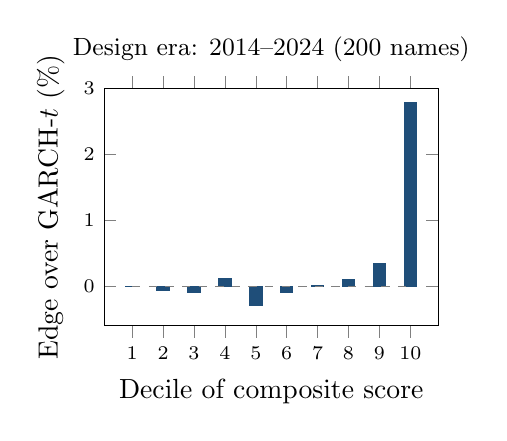
\begin{tikzpicture}
\begin{axis}[width=0.48\textwidth, height=4.6cm, ybar, bar width=4.5pt,
  xlabel={Decile of composite score}, ylabel={Edge over GARCH-$t$ (\%)},
  xtick={1,2,3,4,5,6,7,8,9,10}, ymin=-0.6, ymax=3.0,
  title={\small Design era: 2014--2024 (200 names)}, tick label style={font=\scriptsize}]
\addplot[fill=npblue, draw=npblue] coordinates
  {(1,-0.004)(2,-0.066)(3,-0.101)(4,0.119)(5,-0.287)(6,-0.089)(7,0.012)(8,0.108)(9,0.347)(10,2.787)};
\draw[gray,dashed,thin] (axis cs:1,0) -- (axis cs:10,0);
\end{axis}
\end{tikzpicture}\hfill
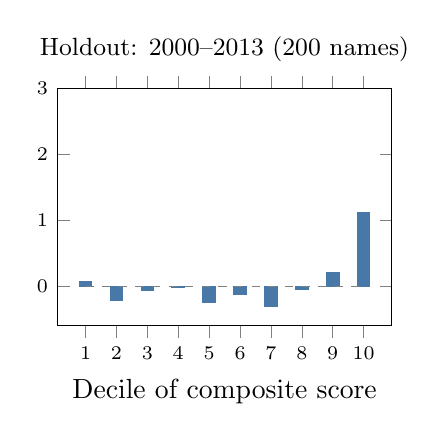
\begin{tikzpicture}
\begin{axis}[width=0.48\textwidth, height=4.6cm, ybar, bar width=4.5pt,
  xlabel={Decile of composite score},
  xtick={1,2,3,4,5,6,7,8,9,10}, ymin=-0.6, ymax=3.0,
  title={\small Holdout: 2000--2013 (200 names)}, tick label style={font=\scriptsize}]
\addplot[fill=npmid, draw=npmid] coordinates
  {(1,0.078)(2,-0.222)(3,-0.068)(4,-0.012)(5,-0.253)(6,-0.12)(7,-0.309)(8,-0.053)(9,0.207)(10,1.123)};
\draw[gray,dashed,thin] (axis cs:1,0) -- (axis cs:10,0);
\end{axis}
\end{tikzpicture}
\caption{The frontier in and out of era, by decile of the composite
misspecification score. Left: the design era (2014--2024). The top
decile carries $+2.79\%$ at per-date DM $8.9$, while deciles one through
nine sit within $\pm0.35\%$. Right: the composite score run
once on 2000--2013 CRSP data. The top decile carries $+1.12\%$ at
per-date DM $2.51$ over 1{,}465 dates. The threshold shape (edge
concentrated in the top decile, near zero elsewhere) survives an
untouched era containing the 2008 crisis.}
\label{fig:holdout}
\end{figure}
The overall
signal--edge correlation is low (0.05--0.10) because the relationship
is a threshold nonlinearity, so the top-decile
Diebold--Mariano statistics are the appropriate summary.

\subsection{The frontier across universes}

\begin{table}[t]
\centering
\begin{threeparttable}
\caption{The frontier across universes. Ratio $=$
nonparam/GARCH-$t$ pinball ($<1$: nonparametric wins). All fits
standalone per asset except where noted.}
\label{tab:universes}
\footnotesize\setlength{\tabcolsep}{4pt}
\begin{tabular}{llccl}
\toprule
Universe & Segment & Ratio & Resid.\ kurt. & Significance \\
\midrule
FX (24 pairs) & majors (7) & 1.019 & 39 & GARCH, pooled DM $-13.7$ \\
 & EM (10) & 1.013 & 8 & GARCH, pooled DM $-9.5$ \\
 & crisis (7) & 0.973 & $\sim$1915 & nonparam, pooled DM $4.12$ \\
 & \quad USDARS & 0.880 & 3298 & DM $2.86$, $p=.002$ \\
 & \quad USDEGP & 0.857 & 1920 & DM $3.80$, $p=.0001$ \\
\midrule
Country indices (26) & developed (8) & 1.007 & 4.7 & 0 nonparam wins \\
 & emerging (10) & 1.012 & 5.3 & 0 nonparam wins \\
 & frontier (8) & 0.993 & 10.0 & 4 significant wins\tnote{a} \\
\midrule
Cross-asset (43) & vol indices & $\sim$0.987 & 32.8 & 3/3 significant \\
 & Baltic freight & 0.846 & --- & DM $9.4$ (calib.\ fails) \\
 & IG credit OAS & 0.960 & --- & DM $2.3$ (indep.\ fails) \\
\multicolumn{5}{l}{\quad 13/43 significant wins overall, corr(log kurt, edge) $= 0.43$} \\
\midrule
Korea 2026 (23) & all types & 1.01--1.12 & 4--13 & GARCH wins all, DM $-2.5$ to $-5$ \\
\bottomrule
\end{tabular}
\begin{tablenotes}\footnotesize
\item[a] Sri Lanka (DM 3.20), Kenya (3.52), Pakistan (2.38), Nigeria (2.06). Exploratory: only Kenya survives the 93-comparison
familywise adjustment (Online Appendix Table~OA.4). Cross-index corr(log residual kurtosis, edge) $= 0.53$.
Philippines is the exception (GARCH wins despite kurtosis 13.6),
illustrating that kurtosis is neither necessary nor sufficient.
\end{tablenotes}
\end{threeparttable}
\end{table}

Table~\ref{tab:universes} shows the same axis at work across markets.
The decisive standalone wins are the hyperinflation and capital-control
currencies, the Argentine peso and the Egyptian pound, 12--14\% better
and individually significant, whose residual kurtosis ($\sim$2000--3300)
sits two orders of magnitude above anything GARCH-$t$ was built to
absorb. Twenty-six country indices trace a gradient that tracks residual
kurtosis rather than the development label, and forty-three cross-asset
instruments extend the pattern into rates, commodities, and credit. The
Korea-2026 crash is the negative control: a price crash under circuit
breakers censors the return but leaves residual kurtosis ordinary, and
GARCH-$t$ correctly wins all twenty-three assets, so the frontier tracks
residual shape and not price turbulence. The instrument-level entries are
exploratory, and under a Holm step-down over the 93 comparisons (Online
Appendix Table~OA.4) seven survive. The aggregate crisis-tier FX
statistic (DM 4.12) and the cross-universe kurtosis--edge gradients are
the evidence this section rests on. A frequency dimension is left to
future work: the five daily crypto series show no edge, while at hourly
frequency the picture inverts.

\subsection{Regime dependence and model selection}
\label{sec:gate}

In the amortized panel the absolute edge grows about fourfold with
turbulence, from 0.0059 in the calmest realized-vol quintile to 0.0247 in
the most turbulent, and both nonparametric estimators beat GARCH in every
quintile. Gating, running GARCH on calm days and the nonparametric model
when the score is high, does not improve on continuous use of the
flexible model: a classifier gate routes $90.5\%$ of days to the
nonparametric model and matches always-nonparametric exactly, and a
regression gate on the edge magnitude \citep{giacominiwhite2006} still
converges to it. This is consistent with Table~\ref{tab:frontier}: the
conditional mean of the loss differential is positive where the score is
high and indistinguishable from zero elsewhere, so no state pays to
select the parametric quantile, and the per-day oracle gap ($4.4\%$) is
unreachable because which day the tail event lands is unpredictable from
prior-day state. The amortized setting therefore uses the nonparametric
model throughout; the residual-hybrid is the choice where a guaranteed
$\ge$GARCH floor is wanted, with the score as a monitor
(Section~\ref{sec:applications}).

%% ===== FRTB EVALUATION =====
\section{VaR and Expected Shortfall forecast evaluation}\label{sec:frtb}

\subsection{Head-to-head accuracy and significance}

Table~\ref{tab:frtb} reports the full comparison on 140 CRSP names (155k observations, 1{,}108 dates).

\begin{table}[t]
\centering
\begin{threeparttable}
\caption{FRTB comparison: average pinball loss (twelve quantile levels),
ES$_{97.5}$ calibration, and 99\% exception tests. 140 CRSP names, 155k
test observations.}
\label{tab:frtb}
\small\setlength{\tabcolsep}{4.5pt}
\begin{tabular}{lcccc}
\toprule
Model & Avg.\ pinball & ES$_{97.5}$ pred.\ vs realized & Breach$_{99}$ & Kupiec$_{99}$ $p$ \\
\midrule
\emph{Ideal value} & \emph{(smaller better)} & \emph{(pred.\ $=$ realized)} & \emph{1.00\%} & \emph{$>0.05$ (pass)} \\
\midrule
Residual-hybrid (GBM) & \textbf{0.3551} & $-6.37$ / $-5.83$ & 1.09\% & 0.00 \\
\quad $+$ EVT tail & 0.3555 & $-6.92$ / $-5.91$ & 0.91\% & 0.00 \\
GARCH(1,1)-$t$ & 0.3561 & $-6.69$ / $-5.65$ & 1.06\% & 0.026 \\
GJR-GARCH-skew-$t$ & 0.3562 & $-6.58$ / $-5.84$ & 1.05\% & 0.062 \\
GARCH-FHS (per-name) & 0.3562 & $-6.61$ / $-5.84$ & 1.11\% & 0.00 \\
GARCH-FHS (pooled) & 0.3566 & $-6.90$ / $-5.67$ & 0.99\% & 0.79 \\
GARCH-FHS (rolling 500d) & 0.3569 & $-6.53$ / $-5.98$ & 1.09\% & 0.00 \\
EWMA (RiskMetrics) & 0.3606 & $-5.52$ / $-5.63$ & 1.63\% & 0.00 \\
Historical simulation & 0.3619 & $-7.21$ / $-6.86$ & 0.84\% & 0.00 \\
\bottomrule
\end{tabular}
\begin{tablenotes}\footnotesize
\item All columns come from a single common-sample run, provided in
the replication package: the 140 CRSP names with the most
complete history (at least 1{,}500 return observations each), over the
common 1{,}108 test dates (155k asset-days), so each per-name exception
test is adequately powered. The rolling-FHS burn-in then trims the same
early dates from all models identically.
Predicted ES is the numerical tail integral
$\alpha^{-1}\!\int_0^\alpha Q(u)\,du$: closed forms for the $t$ and
normal entrants, 200-node integration of the Hansen skew-$t$ inverse
CDF, and a matched 20-node midpoint rule for the empirical quantile
models and for the residual-hybrid, whose VaR and ES are both read from
one monotonized min-envelope curve $Q^{*}=\min\{$body$,$EVT$\}$. A three-node tail-quantile average, a common shortcut,
understates predicted ES by 2--6\% relative to this integral.
Diebold--Mariano vs the residual-hybrid: GARCH-$t$ 5.0, GJR-skew-$t$ 5.0,
FHS pooled 6.2, per-name 5.2, rolling 5.7, HS 7.5, EWMA 8.7 (all
$p\approx0$, rounded, and stable across reruns). The EVT variant
concedes 0.0004 pinball (DM ${\approx}6$) to the first row, the raw
residual-hybrid without the tail, as the price of that tail. The 90\% MCS contains the
raw residual-hybrid alone, and CAViaR (separate common-sample run)
statistically ties it.
\item The ES columns are a diagnostic, not a ranking:
``realized'' is the mean return below each model's own VaR, so
the conditioning set is model-dependent, and under the numerical integral
each fat-tailed entrant exceeds its own-tail comparator by 9--22\%.
The joint Fissler--Ziegel score of the FZ0 re-scoring is the ranking
criterion for ES.
\item GJR-skew-$t$ row: Hansen inverse CDF with the fitted
$\eta,\lambda$ (median $4.2$, $-0.015$), validated against the
symmetric-$t$ limit and against an independent reference implementation.
\item Exception columns are pooled panel diagnostics: at 155k
observations a breach-rate deviation of $\pm0.1$ points rejects in
either direction (the EVT variant's 0.91\% sits on the conservative
side, pooled FHS happens to land at 0.99\%), so pooled $p$-values are
reported, not leaned on. The regulatory reading is the per-asset and
date-clustered restatement (Online Appendix Figure~OA.2): per asset the
EVT-tailed residual-hybrid passes Kupiec at 99\% for $84\%$ of names and
Christoffersen for $86\%$, and the date-clustered test passes at 99\% ($t=1.01$) and marginally at 97.5\% ($t=1.86$) while the raw residual-hybrid is rejected ($t=4.5$): the tail stages carry the regulatory
calibration, and the 2008-era re-run confirms it out of era.
At 97.5\% the split-conformal recalibration is the stage that repairs
pooled Kupiec (GBM-recal $p=0.24$).
\end{tablenotes}
\end{threeparttable}
\end{table}

\paragraph{The stress-era replication.} The comparison set was re-run on the pre-committed 2000--2013 holdout panel. Splits follow
Section~\ref{sec:protocol}, so each name's test window runs from
roughly mid-2008 through 2013, the crisis and its aftermath. The
EVT-tailed residual-hybrid passes Kupiec at 99\% for $94\%$ of names and
Christoffersen for $95\%$, with date-clustered $t$-statistics of
$0.17$ at 99\% and $0.35$ at 97.5\%, consistent with nominal at both regulatory levels through the crisis window. Historical simulation, by far the most common method in bank
disclosures \citep{perignonsmith2010}, and EWMA do not survive the same test: historical simulation
breaches at $1.53\%$ against a $1\%$ target (pass rate $61\%$,
date-clustered $t=2.08$) and EWMA at $1.57\%$ ($t=2.83$). GARCH-$t$ is also well calibrated in this era ($94\%$ pass rate), as the frontier predicts. Calibration parity is the norm, and the residual-hybrid's added value in any era is the accuracy edge where the misspecification score is high. The conformal layer, calibrated on pre-crisis data, tilts conservative on the 2000--2013 holdout (breach $2.21\%$ against the $2.5\%$ target, $t=-1.09$, not significant). The safety margin widens when the calibration era is calmer than the test era, and the error runs in the direction regulators prefer.

\paragraph{Non-core comparisons.} Table~\ref{tab:noncore} adds two entrants from outside banks' standard toolkit. SAV-CAViaR, a leading semiparametric academic benchmark, ties the residual-hybrid, and the $90\%$ Model Confidence Set on that run contains exactly these two, so the residual-hybrid ties the strongest non-nested academic rival and significantly beats every model in banks' standard toolkit. The two tied models differ in what they deliver: SAV-CAViaR models one quantile level per fit, produces no ES (the FRTB metric) without an ad-hoc stage, and needs per-name history, so it cannot be applied to new listings; the residual-hybrid produces the full curve and extends to new listings. Pooled exception rejections are not counted against CAViaR, because pooled asset-day tests ignore cross-sectional dependence and overstate rejection for every model, the residual-hybrid included; the date-clustered restatement is the appropriate reading. A neural IQN used as the residual model loses to trees at both tunings (Table~\ref{tab:noncore}): the tail-aware, monotone, conformally recalibrated version narrows the untuned gap by an order of magnitude and repairs the thin tail, but the remaining deficit is still significant, so trees are the stronger tabular estimator and the residual-hybrid's edge does not rest on the choice of shape learner. Two textbook FHS variants, per-name train-constant and per-name rolling 500-day trailing, were run on the identical panel; both lose to the residual-hybrid (DM 5.2 and 5.7, pinball 0.3562 and 0.3569 against 0.3551) and bracket the pooled variant used in Table~\ref{tab:frtb}.

\begin{table}[htbp]
\centering
\begin{threeparttable}
\caption{Non-core comparisons. Each entrant is scored against the residual-hybrid on its own common sample, so loss levels are comparable within a row but not across rows.}
\label{tab:noncore}
\footnotesize\setlength{\tabcolsep}{5pt}
\begin{tabular}{lccccl}
\toprule
Entrant & Loss & Residual-hybrid & DM & Breach$_{99}$ & Verdict \\
\midrule
SAV-CAViaR & 0.3461 & 0.3460 & 0.4 & --- & tie ($p=0.34$) \\
Neural IQN, untuned & 0.3650 & 0.3551 & 13.3 & 3.2\% & loses \\
Neural IQN, tuned\tnote{a} & 0.3638 & 0.3632 & 3.03 & 0.92\% & loses \\
\bottomrule
\end{tabular}
\begin{tablenotes}[flushleft]\footnotesize
\item[a] Tail-aware $\tau$-sampling, monotone rearrangement, and the conformal overlay of Section~\ref{sec:hybrid}.
\item DM is the per-date Diebold--Mariano $t$-statistic against the residual-hybrid; positive favors the residual-hybrid. The $90\%$ Model Confidence Set contains the residual-hybrid alone on the Table~\ref{tab:frtb} run, and the residual-hybrid together with CAViaR on the CAViaR run. Breach rates were not computed for the CAViaR run, which reports one quantile level per fit.
\end{tablenotes}
\end{threeparttable}
\end{table}
The ES columns of Table~\ref{tab:frtb} are diagnostic only. Under the exact tail integral, each fat-tailed entrant's predicted ES exceeds the realized mean below its own VaR, by 9\% (raw residual-hybrid, rolling FHS) to 22\% (pooled FHS). The comparator conditions on each model's own breach set. The joint FZ0 score below is the ES ranking used in this paper.

\paragraph{The joint $(\VaR,\ES)$ score.} Because ES is not elicitable
alone but the pair $(\VaR,\ES)$ is jointly elicitable under the
Fissler--Ziegel class \citep{fissler2016}, the comparison set was also scored under the FZ0 joint score
\begin{equation}
L_{\mathrm{FZ0},\alpha}(r,q,e)=-\frac{1}{\alpha e}\,\mathbb{I}\{r\le q\}(q-r)
+\frac{q}{e}+\log(-e)-1,\qquad e\le q<0,
\label{eq:fz0}
\end{equation}
the $0$-homogeneous member of the class \citep{patton2019}. Lower values are better. On the
large-cap sandbox subset used to fix the score's orientation, a
Gaussian-innovation GARCH is significantly worst at both the 2.5\% and 1\%
levels (DM 5.4 and 6.0): under a jointly consistent score, Gaussian innovations
are clearly inadequate. Among the fat-tailed entrants the FZ0 differences on
large caps are small ($|$DM$|<1.4$), the frontier's own prediction that the
shape edge is flat on well-behaved names. On a high-kurtosis subset the ordering favors the shape-aware forecaster, directionally but not significantly at that width. The pre-specified full-panel run, reported next, settles the magnitudes on the residual-hybrid's own forecasts.

\begin{figure}[t]
\centering
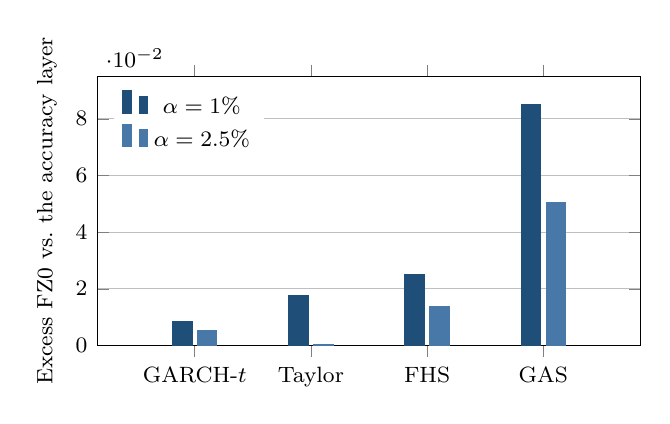
\begin{tikzpicture}
\begin{axis}[width=0.7\linewidth,height=5cm, ybar, bar width=7pt,
  ymin=0, ymax=0.095, ylabel={Excess FZ0 vs.\ the accuracy layer},
  symbolic x coords={GARCH-$t$,Taylor,FHS,GAS}, xtick=data,
  enlarge x limits=0.28, ymajorgrids,
  legend style={font=\footnotesize,at={(0.03,0.97)},anchor=north west,draw=none},
  tick label style={font=\footnotesize}, label style={font=\footnotesize}]
\addplot[fill=npblue,draw=npblue] coordinates {(GARCH-$t$,0.00848)(Taylor,0.01748)(FHS,0.02517)(GAS,0.08514)};
\addplot[fill=npmid,draw=npmid] coordinates {(GARCH-$t$,0.00545)(Taylor,0.00024)(FHS,0.01370)(GAS,0.05030)};
\legend{$\alpha=1\%$,$\alpha=2.5\%$}
\end{axis}
\end{tikzpicture}
\caption{Joint (VaR, ES) FZ0 loss of each benchmark in excess of the
residual-hybrid's accuracy layer (the EVT-tailed variant without the
conformal shift), on the full 200-name panel. A positive bar
means worse than the accuracy layer. The accuracy layer (the zero baseline) attains the
lowest FZ0 at both regulatory levels, beating GARCH-$t$ (DM $4.8$ at
$1\%$, $5.1$ at $2.5\%$) and FHS (DM $4.9$), together with the two
FZ-estimated dynamic-ES benchmarks fitted per name by multi-start FZ0
minimization, the GAS of \citet{patton2019} (DM $9.5$ and $8.6$) and the
ES-CAViaR of \citet{taylor2019} (DM $3.6$ at $1\%$, a tie at $2.5\%$). SAV-CAViaR, scored on its own common sample (Table~\ref{tab:noncore}), ties the accuracy layer and is omitted here; the conformal-overlay variant, which concedes FZ0 at $2.5\%$, is discussed in the text.}
\label{fig:fz0}
\end{figure}

On the full 200-name panel ($221.6$k test asset-days), VaR and ES are read from the coherent min-envelope curve $Q^{*}$ and per-date DM inference is used throughout. The residual-hybrid's \emph{accuracy layer}, the EVT-tailed variant with no conformal shift, attains the lowest FZ0 at both regulatory levels. At 1\% it beats GARCH-$t$ (DM 4.8) and FHS (DM 4.9), the two standard benchmarks the accuracy claim rests on. At 2.5\% it again wins over GARCH-$t$ (DM 5.1). The two FZ-estimated dynamic $(\VaR,\ES)$ models a referee would turn to next are the one-factor score-driven GAS of \citet{patton2019} and the ES-CAViaR of \citet{taylor2019}. Each is estimated per name on the same panel by minimizing the same FZ0 loss, and under a three-start optimizer both converge for all $200$ names, so the single-start instability of an earlier attempt does not arise. The accuracy layer beats the GAS at both levels (DM 9.5 at 1\%, 8.6 at 2.5\%), and it beats the Taylor model at 1\% (DM 3.6) while tying it at 2.5\% (DM 0.1), the near-tie the fat-tailed benchmarks all show at 2.5\% where the shape edge is thin.

This ranking survives the annual walk-forward refit of Section~\ref{sec:calendarleak}: re-estimating every stage at each January-1 cutoff and re-scoring the 2020--2024 panel, the accuracy layer keeps the lowest FZ0 at both levels, beating GARCH-$t$ and FHS by DM 3.6 and 2.7 at 1\% and 3.1 and 2.6 at 2.5\% (one-sided $p<0.005$). Refitting narrows these margins without closing them, unlike the average pinball edge, which closes under the same refit.

The accuracy layer is thus one configuration that attains the lowest FZ0 at both levels and passes the aggregate date-clustered exception test at 99\% and marginally at 97.5\%. Per-name diagnostics show residual cross-sectional calibration heterogeneity (84\% and 86\% pass rates at 99\%, Online Appendix Figure~OA.2). The one failed test is the pooled 155k-observation Kupiec at 97.5\%, which at this sample size rejects very small deviations. The frontier concentrates the joint-score
edge as it does the pinball edge: the top misspecification decile
carries DM 2.4 at the 1\% level against DM 0.2 in the panel bulk.
Adding the conformal shift at 97.5\%, whose calibration split includes
the 2020 crash, widens the band out of era (breach $1.66\%$ against the $2.5\%$ target) and gives back the FZ0 advantage there. The static-overlay variant loses to GARCH-$t$ on the 2.5\% joint score (DM $-2.0$), and the concession is largest in the top misspecification decile, where the static shift's joint-score deficit reaches DM $-7.1$.

The coverage
property costs sharpness under
a strictly consistent score, and its error direction is conservative
(wider bands, fewer breaches than nominal). Where the conservative
coverage margin is valued, the shift is kept; where FZ0 efficiency is
the criterion, the EVT tail is run alone, and it passes the exception
tests on its own (Online Appendix Figure~OA.2).

Most of the concession reflects a frozen margin. The adaptive form of the shift \citep{gibbs2021aci}, updated daily from the panel breach frequency, shrinks the margin out of era (from $-0.35$ to $-0.10$, breach $1.83\%\to2.06\%$) and erases the overall concession. The adaptive variant ties GARCH-$t$ on 2.5\% FZ0 (DM $-0.3$). The top-decile cost survives the adaptive shift too, at $-4.8$ and $-6.0$ for the two update rates against the static shift's $-7.1$, the price of a margin where the bands are widest. The static shift also worsens per-name coverage (Kupiec$_{97.5}$ pass rate 47\%, against 72\% unshifted and 69\% adaptive), because over-coverage fails the test from the other side. Each ``lowest FZ0'' statement refers to the accuracy layer.

\paragraph{Direct ES calibration backtests.} Because exception counts test VaR and not ES,
two direct ES calibration backtests, the McNeil--Frey exceedance-residual test \citep{mcneilfrey2000} and the Acerbi--Sz\'ekely $Z_2$ statistic \citep{acerbi2014backtesting}, complement the jointly consistent FZ0 loss above. \citet{noldeziegel2017elicitability} and \citet{bayer2022esr} draw the
distinction between backtesting the calibration of an ES forecast and comparing
forecasts through a joint score. Both are computed on the residual-hybrid's own min-envelope forecasts over the same $200$-name panel, with a stationary block bootstrap over the $1{,}108$ test dates (Online Appendix). The Gaussian filter is worst on each ES metric, and among the fat-tailed entrants no single model dominates each diagnostic. The residual-hybrid has the $Z_2$ closest to zero at $1\%$ and ties GARCH-$t$ at $2.5\%$, and the residual-hybrid and GARCH-$t$ are the two models that pass the $1\%$ Kupiec test. On the McNeil--Frey residual, FHS, which targets the empirical tail directly, is closest to zero. The calibration tests show that the residual-hybrid's tail is well calibrated. The comparative result is the FZ0 loss, where the edge over GARCH-$t$ and FHS is significant at both levels.

\subsection{The ten-day horizon: a direct multi-day extension}

The multi-day results come from a direct amortized model trained on
$h$-day cumulative returns; the residual-hybrid of Algorithm~1 is a
one-day architecture, and no ten-day claim attaches to it. At the FRTB
ten-day liquidity horizon (CRSP 2014--2024) its pinball edge over
$\sqrt{h}$-scaled GARCH grows from $\sim$0.4\% at $h=1$ to $\sim$1.4\% at
$h=10$ and holds in the 2020--2022 stress window (Online Appendix
Figure~OA.3). The ten-day tail advantage is real in that era but does not
survive the pre-committed 2000--2013 rerun: out of era the two methods
tie on accuracy (direct edge $+0.49\%$, DM 0.07) and the calibration
verdict reverses, with $\sqrt{h}$-scaled GARCH-$t$ almost exactly
calibrated through the crisis while the direct tail under-states it. In a
2008-type era the direct ten-day model should therefore be run with the
$\sqrt{h}$-scaled parametric number alongside it as a conservative
envelope. The ten-day evidence is therefore mixed; the full
tables are in the Online Appendix.

\subsection{Cross-asset evidence}

Across the 43-instrument sweep the relationship is heterogeneous. The volatility indices (VIX, V2X, VVIX) and Baltic freight post the largest accuracy gains and survive the multiplicity adjustment (Online Appendix Table~OA.4), but their calibration is open. VIX's breach-independence is marginal (one-sided $p=0.041$), and credit and Baltic freight fail it, so all are reported as accuracy edges rather than calibrated wins. An apparent electricity win reversed once the return transformation was corrected for near-zero prices. The GPD tail is left off for some
volatility indices, where the raw body already covers, by the coverage-based activation rule of
Section~\ref{sec:hybrid}. Instrument-level results and diagnostics are
collected in the Online Appendix.

\paragraph{The scale--shape decomposition.} Against a Realized GARCH \citep{hansen2012realized} fitted on intraday data, the daily-data core concedes FZ0 at both levels (DM $6.2$ and $4.5$). Re-fitting the shape learner, EVT tail, and score on the realized residuals, however, leaves the score within noise. On large caps the frontier is therefore largely daily-scale misspecification. Where intraday data are unavailable or too sparse to build a realized measure (new listings, illiquid names, many cross-asset instruments), the daily score is the version of the diagnostic that can be computed (Online Appendix).

%% ===== APPLICATIONS =====
\section{Extensions and implications}\label{sec:applications}

\noindent The full estimation and forecasting pipeline is stated in the Online Appendix.

\paragraph{Using the score.} The score is available \emph{ex ante}: a
risk manager computes today's value from today's residuals and uses it
for tomorrow's forecast. Its role is to stratify, not to switch models
day by day, because the per-day oracle gap is not forecastable from
prior-day state and a learned gate collapses to always-nonparametric
(Section~\ref{sec:gate}). The one setting in which it drives a switch is
the per-name standalone model, where nonparametric quantiles underperform
on calm days. As a monitor it is cheap, since its input is the trailing
residual window the scale stage already produces, and it is a slow state
that need not be watched daily. On capital, the residual-hybrid is a
one-day single-name VaR/ES forecaster of the kind that feeds an internal
model, not the ten-day portfolio-level stressed ES that sets the FRTB
charge; the paper makes no capital-release claim, because the
predicted-versus-realized ES wedge conditions on each model's own breach
set and no defensible arithmetic converts it to capital
\citep{bcbs2019frtb}. The narrower implication is that the ES-based
component of the charge scales with the ES forecast.

\paragraph{Cold-start risk for new listings.} The amortized model in its
characteristics-only form is the only entrant here that can produce a
conditional risk forecast for an asset with no return history. An IPO or
newly listed ETF gets day-one quantiles from its characteristics and
first ticks, because the model was trained on the pooled (state, loss)
pairs of hundreds of other names; the residual-hybrid of
Section~\ref{sec:hybrid} attaches once a scale filter is estimable. The
amortized forecast beats own-history benchmarks at each listing age, and
the edge is largest when the name is young ($\sim$6--10\% of pinball in
the first trading month). The ablation in Section~\ref{sec:gbcmethod}
traces the handover from characteristics to the name's own realized
volatility as its history lengthens.

% Trading implications and scenario generation are discussed in the Online Appendix.

\section{Conclusion}\label{sec:limitations}

A fixed-shape parametric filter is hard to beat where its shape assumption holds, and for most assets on most days it holds well. The flexible model's advantage is concentrated in a small set of high-stress states identified by the real-time misspecification score. The decomposition attributes most of this advantage to post-outlier variance overstatement by the standard GARCH filter; a smaller but significant component remains after replacing it with a jump-robust scale, and is conditional-shape information a robust scale leaves intact. An estimator that exploits both components, while showing no detectable accuracy loss relative to the benchmark elsewhere, improves on the accuracy of the market-risk models in standard use when judged by one-day diagnostics at the FRTB backtesting levels, at calibration parity with the best of them and short of the desk-level approval a full internal model must pass. Because the estimator pools its residual model across names, it also forecasts tail risk for assets with no history of their own, forecasting new listings from their first day as no per-asset model can.

These conclusions carry qualifications. The score is predictive, not a necessary or sufficient condition: high residual kurtosis coincides with ties in some markets, and in credit and freight the accuracy edges sit alongside open calibration. The shape component is the smaller part of the edge, since the decomposition attributes most of it to daily-scale misspecification that a jump-robust or realized-variance scale removes (Section~\ref{sec:frtb}), and what survives is real but modest. Where intraday data are too sparse to build a realized measure, the daily model and its score remain the available tool. And the score is a monitor, not a day-to-day switching rule, since the day-ahead oracle gap is largely unforecastable (Section~\ref{sec:gate}).
Distributional uncertainty around these VaR and ES forecasts and the multivariate portfolio tail are left to future work.

\section*{Funding}
This work was supported by the Northwestern University Department of
Statistics and Data Science [Undergraduate Research Fellowship Grant,
2026].

\section*{Acknowledgments}
I thank Wenxin Jiang for his advice and guidance throughout this
research, and seminar participants and colleagues for comments. All
errors are mine.
AI assistance (Anthropic's Claude) was used in drafting, editing, and
code development; the author designed the research, verified all
results, and is responsible for the content.

\section*{Conflict of interest}
The author declares no conflicts of interest.

\section*{Ethics statement}
This study uses licensed secondary market data (CRSP/WRDS and
Bloomberg) under the terms described in the data availability
statement. It involves no human subjects and required no ethics
approval.

\section*{Data and code availability}
\addcontentsline{toc}{section}{Data and code availability}
A public replication package at
\href{https://github.com/sean-qin-usa/downside-risk-paper}{\texttt{github.com/sean-qin-usa/downside-risk-paper}}
covers every WRDS-based table and figure in this paper and preserves
the Bloomberg-based exhibits as run from their derived series. It
provides estimation code for all stages of the estimator
(\eqref{eq:garch}--\eqref{eq:hybrid}), the misspecification score
\eqref{eq:score}, the FRTB comparison, the generative-posterior and SBC
routines, and the walk-forward schedule, seeds, and hyperparameter grids
referenced in the text, together with a mapping from each table and
figure to the script and result file that produce it. Return data
derive from CRSP, Bloomberg, and OptionMetrics under the author's
institutional licenses and cannot be redistributed; the package
includes the code to rebuild each panel from those sources, the derived
non-proprietary series, and a synthetic example dataset on which the
full pipeline runs end-to-end without licensed data. The holdout's
frozen specification, including its written-in-advance predictions, is
recorded in the package alongside the design-era pipeline so that the
two can be compared line by line. A citable archival snapshot (Zenodo
DOI) will be minted for the accepted version.

\begingroup
\parindent 0pt\parskip 1ex
\renewcommand{\enotesize}{\normalsize}
\theendnotes
\endgroup

%% ===== BIBLIOGRAPHY =====
\bibliographystyle{apalike}
\bibliography{refs_v3}

% Proofs and supplementary exhibits are in the Online Appendix.

\end{document}
